\chapter{BMF Rank Selection by Minimum Description Length}
\chaptermark{Rank Selection by MDL}\label{chap:RankMDL}
The possibility to derive a Boolean factorization by means of  numerical optimization methods is a promising theoretically founded alternative to the greedy heuristic, generally applied for \ref{eq:BoolMF} (cf.\@ Section~\ref{sec:ZS:GreedyApproach}). Yet, we also wish to provide a solution to the well researched topic of model selection in Boolean matrix factorization by virtue of \textsc{PAL-Tiling}.  
%one of the most  then we would still face a serious preference bias. This bias concerns the model selection with respect to the number of expected clusters and is generally a crucial question in clustering. However, while the \ref{eq:BoolMF} optimization is not particularly theoretically founded (so far), the determination of the optimal rank in \ref{eq:BoolMF} is. 
However, this objective is difficult to delineate: where to draw the line between structure and noise? One possibility is to apply the \emph{Minimum Description Length} (MDL) principle as proposed by \cite{miettinen2014mdl4bmf} to reduce the considerations into one: exploit just as many regularities as serves the compression of the data. Here, regularities indicate the structural part, 
the similarities between observations which establish a cluster. The description length counterbalances the complexity of the model (the amount of derived clusters) with the fit to the data, measured by the size of the encoded data using the model. Decisive for the feasibility of extracted components is the definition of the encoding. 

\cite{miettinen2014mdl4bmf} evaluate several encodings with respect to their ability to filter a planted structure from noise. Candidate clusters are created by the Boolean matrix factorization \textsc{Asso} and are afterwards selected such that a specified description length is minimized. Another framework proposed by \cite{lucchese2014unifying} greedily selects the clusters which directly minimize the description length. Most recently, \cite{karaev2015getting} propose another greedy scheme with focus on a setting where noise effects more likely flip a one to zero than the other way round. All these methods are capable to identify the underlying clusters in respectively examined settings. By and large, the experiments indicate however that the quality considerably varies depending on the distribution of noise and characteristics of the dataset~\citep{miettinen2014mdl4bmf,karaev2015getting}.  Our main contributions are:
\begin{itemize}
    \item We facilitate the application of the framework \emph{PAL-Tiling} to optimize a description length having an approximation which is suitable for the optimization via PALM, \item we algorithmically integrate the built-in regularization of the model complexity by MDL in order to derive factorizations which do not use more tiles than necessary,
    \item we propose two algorithms as specifications of \textsc{PAL-Tiling}: one applying $\ell 1$-regularization on the matrix factorization (\textsc{Panpal}) and one employing an encoding by code tables as proposed by \cite{siebes2006item} (\textsc{Primp}). 
\end{itemize}
 
%We assess the algorithms' ability to filter the \textit{true} underlying structure from the noise. Therefore, we compare various performance measures in a controlled setting of synthetically generated data as well as for real-world data. We show that \textsc{Primp} is capable of recovering the latent structure in spite of varying database characteristics and noise distributions. In addition, we visualize the derived categorization into clusters by means of images, showing that our conducted minimization procedure of \textit{PAL-Tiling} yields interpretable groupings. 
%=============================
% The MDL Principle
%=============================
\section{MDL Principle}
MDL is introduced by \cite{rissanen1978modeling} as an applicable version of Kolmogorov complexity~\citep{li2008introduction,grunwald2007minimum}.
The learning task to find the best model according to the MDL principle is given by the following minimization problem 
\begin{align*}
    	\min_M&\ L(M) = L^D(M) + L^M(M) &\text{s.t. } M\in\mathcal{M}.
\end{align*} 
The function $L$ denotes the description length, which is composed of the compression size of the database in bits $L^D(M)$ (using model $M$ for the encoding) and description size in bits of the model $M$ itself $L^M(M)$.
Specifications of this task differ in the definition of the encoding which defines in turn the set of considered models $\mathcal{M}$. 
%Typical models for tilings are given by the factorizations which satisfy the constraints
%\[
%	\mathcal{M} = \{(X,Y)\in \{0,1\}^{n\times r}\times\{0,1\}^{m\times r}\mid c(X,Y,N) \leq 0\ \forall c\in \mathcal{C}, r\in\mathcal{R}\}.
%\]
%-----------------------------------
% MDL for itemset compression
%-----------------------------------
\subsection{MDL for Pattern Mining}
The minimum description length is suitable to tackle the problem of pattern explosion, arising in practical applications of pattern mining. The output of frequent pattern mining algorithms is sensitive to the minimum support threshold, defining the meaning of the word \emph{frequent}. If this threshold is set too high, then only a few patterns are returned, reflecting nothing but common knowledge. A small decrease in the minimum support can result however in the output of a vast amount of patterns, whereby most of them are redundant as well. The minimum description length is applicable to select a set of patterns, giving a succinct description all frequent patterns.   

An encoding which is successfully applied in this respect uses code tables  as proposed by~\cite{siebes2006item}. 
The two-columned code table assigns optimal prefix-free codes to a set of patterns: itemsets are listed on the left and assigned codes on the right. Such a dictionary from itemsets to code words can be applied to databases similarly as code words to natural language texts. However, the usage of codes for patterns in a transaction is not as naturally defined as for words in a text. Patterns are not nicely separated by blanks and the possibilities to disassemble a transaction into patterns are numerous. Therefore, we require for every transaction the indication of those patterns  which are used for the transaction's encoding. This is modeled by the function $cover$, which partitions items indicated in a transaction into patterns of the code table. 

Let $CT=\{(\mathcal{X}_s,C_s)|1\leq s\leq r\}$ represent a code table of $r$ patterns $\mathcal{X}_s\subseteq\{1,\ldots,n\}$ and codes $C_s$. Theorem 5.4.1 in \cite{cover2012elements} states that for any distribution $P$ over a finite set $\Omega$, an optimal set of prefix-free codes exists such that the number of required bits for the code of $x\in\Omega$ is approximately
\begin{equation*}
	codelength(x) \approx -\log(P(x)).
\end{equation*}
Desiring that frequently used codes are shorter in size, \cite{siebes2006item} introduce the function $usage$ that maps a pattern to the number of transactions which use it for their cover,
\[usage(\mathcal{X}_s)=|\{j\in\{1,\ldots,m\}\mid \mathcal{X}_s\in cover(CT,D_{j\cdot})\}|.\] 
The probability mass function over all itemsets $\mathcal{X}_s$ in the code table  is defined as
\begin{align}\label{eq:krimpCodeProb}
P(\mathcal{X}_s) = \frac{usage(\mathcal{X}_s)}{\sum_{1\leq t \leq r}usage(\mathcal{X}_t)}.
\end{align}
This implies that $codelength(\mathcal{X}_s)=-\log P(\mathcal{X}_s)$. The data matrix is encoded by a transactionwise concatenation of codes, denoted by the cover, i.e., transaction $D_{j\cdot}$ is encoded by a concatenation of codes $C_s$ with $\mathcal{X}_s\in cover(CT,D_{j\cdot})$. Therefore, code $C_s$ occurs $usage(\mathcal{X}_s)$ times in the encoded dataset. The size of the data description is then computed as
\begin{align*}
	L^D_{\mathsf{CT}}(CT)
    &=-\sum_{1\leq s\leq r} usage(\mathcal{X}_s) \cdot \log(P(\mathcal{X}_s)).
\end{align*}
The description of the model, the code table, requires the declaration of codes $C_s$ and corresponding patterns $\mathcal{X}_s$. Code $C_s$ has a size of $-\log\left(P(\mathcal{X}_s)\right)$ and a pattern is described by concatenated standard codes of contained items. Standard codes arise from the code table consisting of singleton patterns only, where the usage of singleton $\{i\}$ for $i\in\{1,\ldots,n\}$ is equal to its support $|D_{\cdot i}|$. In conclusion, the description size of the model is computed as  
\begin{align*}
	L_{\mathsf{CT}}^M(CT)
    &= -\sum_{\substack{1\leq s\leq r \\ usage(\mathcal{X}_s)>0}}\left(\log\left(P(\mathcal{X}_s)\right) +\sum_{i\in \mathcal{X}_s}\log\left(\frac{|D_{\cdot i}|}{|D|}\right)\right).
\end{align*}
Note that an efficient computation of the description length employs the possibility to calculate code lengths without realizations of actual codes.
We further remark that the function $L_{\mathsf{CT}}$ originally uses the logarithm with base two. Here, we implicitly reformulate this description length by substituting with the natural logarithm. This is equivalent to multiplying the function by a constant which is negligible during minimization. In return, using the natural logarithm will shorten the derivations in Section~\ref{sec:MDL:primp}.

\cite{siebes2006item} use a heuristic cover function in the algorithm \textsc{Krimp} which employs a specified, static order on patterns. For every transaction, the cover function returns a partition of the transaction by the following routine: iterating through all patterns of the code table in the given order, add a pattern to the transactions' cover whenever the transaction supports the pattern. Remove the items belonging to a selected pattern from the transaction and continue the pattern traversion. This way, the usage of a pattern is smaller than or equal to its support.
The determination of patterns contained in the code table is performed by another greedy procedure in \textsc{Krimp}. An input set of frequent patterns -- the code table candidate set -- is traversed in another static order, adding a candidate pattern to the code table whenever that improves the compression size. Additionally, pruning methods are proposed to correct the selection of patterns in the code table.

\textsc{Slim}~\citep{smets2012slim} differs in its candidate generation, which is   dynamically implemented according to an estimated compression gain and dependent on the current code table. This strategy typically improves the compression size, but mainly reduces  the  amount of returned patterns.  
Both approaches consider a vast amount of candidates until the best set of patterns is determined. Time consumption is dominated by computing the usage for each evaluated candidate.
\textsc{SHrimp} \citep{hess2014shrimp} exploits the indexing nature of trees in order to efficiently identify those parts of the database which are affected by an extension of the code table.
\cite{siebes2011structure} restrict with the algorithm \textsc{Groei} the code table to a constant number of patterns. They resort to a heuristic beam search algorithm,
but only for tiny datasets, the beam width parameter can be set to a level allowing a reasonably wide enough exploration of the search space, or else the run time explodes.

All these algorithms follow the heuristic cover definition of \textsc{Krimp} which restricts the usage of a pattern to supporting transactions and prohibits a cover by overlapping patterns. As discussed in the context of tiling (cf.\@ Section~\ref{sec:ZS:BooleanMF}), these restrictions result in less succinct descriptions of the dataset, being susceptible to noise. Correspondingly, there are methods adapting the model selection by minimum description length for Boolean matrix factorization.
%---------------------------
% MDL for BMF
%---------------------------
\subsection{MDL for BMF}
The scheme to employ MDL for rank selection is easily adopted from the one used for pattern mining. 
In every iteration, the description length of the current factorization is compared with the description length from the former iteration, having a lower rank. If the current factorization achieves a lower description length, then another factorization with an increased rank is computed and the procedure repeats itself. Otherwise, the factorization of the former iteration is returned. The performance of this method depends on the algorithm computing the factorization of a given rank and on the encoding which determines the description length.

\cite{lucchese2010noise} propose an encoding reflecting sparse data representations; describing matrices only by their positions of ones. Consequently, the model is described with $L^M_{\ell 1}(X,Y)=|X|+|Y|$ bits and the data with $L^D_{\ell 1}(X,Y)=|D-\theta(YX^\top )|$ bits, up to a multiplicative constant. We denote the resulting description length with $L_{\ell 1}(X,Y)=|D-\theta(YX^\top )|+|X|+|Y|$. The algorithm \textsc{Panda} uses a factorization method which adds a tile (outer product) to the current factorization in a two stage heuristic. 
 
\cite{miettinen2014mdl4bmf} argue that the encoding used in \textsc{Panda} is too coarse. They investigate multiple encodings, applying \textsc{Asso} as Boolean factorization method. Their best-performing encoding is called \emph{Typed XOR DtM} encoding. This is based upon the description of $n$-dimensional binary vectors by number and distribution of ones. 
We refer to  the Typed XOR DtM description length as $L_{\mathsf{TXD}}$ and to the corresponding algorithm as \textsc{Mdl4bmf}. The experimental evaluation suggests that \textsc{Mdl4bmf}'s rank estimation is accurate in a setting with moderate noise, i.e., less than $15\%$, and moderate number of planted tiles, i.e., less than 15. It seems to have a tendency to underfit, as opposed to \textsc{Panda}, which returns on some synthetically generated datasets a rank ten times higher than the actual rank.

On the other hand, the heuristic optimization of \textsc{Panda} is applicaple to any objective function. \cite{lucchese2014unifying} enhance the algorithm \textsc{Panda} to a faster version \textsc{Panda+} and empirically evaluate the ability to detect the \emph{true} clustering via various description lengths and optimization algorithms. In the evaluation with respect to synthetically generated datasets, having less than $10\%$ equally distributed noise, \textsc{Panda+} using the Typed XOR description length $L_{\mathsf{TX}}$ is outperforming any other choice. The performance is explained with the direct minimization of the description length in \textsc{Panda+}, opposed to \textsc{Asso}, minimizing only the residual sum of squares.

Another algorithm which tries to incorporate the direct optimization of the MDL-cost measure is \textsc{Nassau}~\citep{karaev2015getting}. Remarking that the formerly proposed algorithms do not reconsider which clusters have been mined at previous iterations, \textsc{Nassau} refines the whole factorization every few steps, employing \textsc{Asso} for the \ref{eq:BoolMF} optimization. The experiments focus on a setting where noise effects which flip a one to a zero are prevalent. In this case, differences to \textsc{Mdl4bmf} are often hard to capture while \textsc{Nassau} typically outperforms \textsc{Panda+}. 

%===================================
% MDL and PAL-Tiling
%===================================
\section{Minimizing the Description Length in PAL-Tiling}
We wish to derive Boolean factorizations minimizing the description length, hoping that the regularization of the model complexity by the MDL principle is suitable to yield factorizations of an appropriate rank. However, most of the proposed description lengths are not continuous, let alone smooth. Therefore, we need to derive  a smooth relaxation of the description lengths we wish to apply in \textsc{PAL-Tiling}. We assume that there exists a factor $\mu\geq 0$ and regularizing function $G$ such that the smooth relaxation of the description length has the form 
\begin{align}\label{eq:MDL:F}
	F(X,Y)= \frac{\mu}{2}\|D-YX^\top \|^2 + \frac{1}{2} G(X,Y).
\end{align} 
Here, the multiplication with one half refers to the traditional formulation of the residual sum of squares in problem~(\ref{eq:NMF}), which shortens the formulation of gradients. 
In order to meet the convergence criteria of PALM, we require the regularizing function $G$ to be a smooth definable function, having partial gradients which are Lipschitz-continuous with moduli $M_{\nabla_YG}(X)$ and $M_{\nabla_XG}(Y)$, such that
\[\|\nabla_XG(X,Y)-\nabla_UG(U,Y)\|< M_{\nabla_XG}(Y)\|X-U\|,\]
and similarly for $\nabla_YG$. From the triangle inequality follows that the Lipschitz moduli of the partial gradients of $F$ are then given as
\begin{align*}
M_{\nabla_XF}(Y) &= \mu\|YY^\top \| + \frac{1}{2}M_{\nabla_XG}(Y)\\ 
M_{\nabla_YF}(X) &= \mu\|XX^\top \| + \frac{1}{2}M_{\nabla_YG}(X).
\end{align*}
%--- ALG Toss MDL ----
\begin{algorithm}[t]
\caption{The tossing function for the application of \textsc{PAL-Tiling} implementing the determination of the rank via MDL.} 
\begin{algorithmic}[1]
  \Function{Toss}{$x,y,D$}
  	\State \textbf{return} $|x|\leq 1\ \mathsf{OR}\ |y|\leq 1$ 
  \EndFunction
\end{algorithmic}
\label{alg:MDL:toss}
\end{algorithm}
We specify the function \textsc{Toss} in Algorithm~\ref{alg:MDL:toss}, which we employ in the framework of \textsc{PAL-Tiling} to determine the rank via the minimum description length principle. Since the regularization of the model complexity by MDL is supposed to yield factorizations which penalizes tiles reflecting noise effects, we employ a very simplistic function \textsc{Toss}. The function solely decides that singleton tiles, consisting of one row or column, are to be disregarded in the factorization. Therewith, we only need a specification of the description lengths and their relaxed objective for the optimization in \textsc{PAL-Tiling}.
%--------------------------------------
% Panpal
%------------------------------------
\subsection{Panpal}\label{sec:MDL:panpal}
The cost measure $L_{\ell 1}$ (as applied by \textsc{Panda}) is easily  integrated into \textsc{PAL-Tiling}. Since the proximal operator ensures that the factor matrices in all steps are nonnegative, the $\ell 1$-norm of the factor matrices equates a simple summation over all matrix entries. Thus, the $\ell 1$-norm is a smooth function on the nonnegative domain of the factor matrices and can be used as regularizing function. We call the resulting algorithm \textsc{Panpal} as it employs the cost measure of \textsc{Panda} in the minimization technique \textsc{PAL-Tiling}:
%\begin{mybox}
\begin{algSpec}[Panpal] \label{algSpec:panpal}
Apply \textsc{PAL-Tiling} with the function \textsc{Toss} from Algorithm~\ref{alg:MDL:toss} and the following functions:
\begin{align*}
    L(X,Y)&=L_{\ell 1}(X,Y) = |D-\theta(YX^\top )|+|X|+|Y| & \textit{(objective)}\\
    F(X,Y)&=\frac{1}{2}\|D-YX^\top \|^2+ \frac{1}{2}(|X|+|Y|) & \textit{(smooth part)}\\
    \nabla_XF(X,Y,D)&=(YX^\top -D)^\top Y+0.5\mathbf{1}& \textit{(partial gradient X)}\\
\nabla_YF(X,Y,D)&=(YX^\top -D)X+0.5\mathbf{1} & \textit{(partial gradient Y)}\\
M_{\nabla_XF}(Y)&>\|YY^\top \| \quad M_{\nabla_YF}(X)>\|XX^\top \| & \textit{(L-moduli)}
\end{align*}
\end{algSpec}
%\end{mybox}
The smooth relaxation $F$ in \textsc{Panpal} is a polynomial function and thus semi-algebraic. Therefore, the optimization of the relaxed objective of \textsc{Panpal} via PALM converges to a local minimum.
%-------------------------
% primp
%-------------------------
\subsection{Primp}\label{sec:MDL:primp}
So far, the cost measure of \textsc{Krimp} has been disregarded in the context of Boolean matrix factorization. Since the traditionally employed cover function is incompatible with overlapping patterns or patterns which cover more items than persistent in the transaction, the task to find the best encoding by code tables is associated with the sub-domain of pattern mining \citep{miettinen2014mdl4bmf,lucchese2014unifying,karaev2015getting}. The definition of the long-established cover function is heuristically determined under the assumption that there is one globally valid cover function which is applicable on all datasets if a suitable code table is found. Although this approach might be favorable in sub-domains like classification or detection of changes in a data stream \citep{vreeken2011krimp,van2008streamkrimp}, it is current best practice in the domain of Boolean matrix factorization to take negative noise into account (see Section~\ref{sec:ZS:BooleanMF}).  
Thus, we break away from the conventional view on the cover function as a predefined instance and regard it as an extrapolation of the mapping from patterns to transactions which is defined by the matrix $Y$. Thereby, we intend to learn a suitable pair of code table and cover function, tailored to the dataset. This is motivated by the following observation.
%-------------------------------
\begin{restatable}{lemma}{lctbmf}\label{thm:CTBMF}
Let $D$ be a data matrix. For any code table $CT$ and its cover function there exists a Boolean matrix factorization $D=\theta(YX^\top )+N$ such that non-singleton patterns in $CT$ are mirrored in $X$ and the cover function is reflected by $Y$. The description lengths correspond to each other, such that 
\[L_{\mathsf{CT}}(CT)=L_{\mathsf{CT}}(X,Y)=L_{\mathsf{CT}}^D(X,Y)+L_{\mathsf{CT}}^M(X,Y),\]
where the functions returning the model and the data description size are given as  
\begin{align*}
	L_{\mathsf{CT}}^D(X,Y)&=-\sum_{s=1}^r |Y_{\cdot s}| \cdot \log(p_s)
       -\sum_{i=1}^n |N_{\cdot i}| \cdot \log(p_{r+i})
       &=L^D_{\mathsf{CT}}(CT)\\
    L_{\mathsf{CT}}^M(X,Y)
    &=\sum_{s:|Y_{\cdot s}|> 0}\left(X_{\cdot s}^\top \mathbf{c}-\log(p_s)\right)
	+\sum_{i:|N_{\cdot i}|> 0}\left(\mathbf{c}_i-\log(p_{r+i})\right)&=L_{\mathsf{CT}}^M(CT).
\end{align*}
The probabilities $p_s$ and $p_{r+i}$ indicate the relational usage of non-singleton patterns $X_{\cdot s}$ and singletons $\{i\}$,
\[
	p_s = \frac{|Y_{\cdot s}|}{|Y|+|N|},\  p_{r+i} = \frac{|N_{\cdot i}|}{|Y|+|N|}.
\]
We denote with $\mathbf{c}\in\R_+^n$ the vector of standard code lengths for each item, i.e., 
\[\mathbf{c}_i=-\log\left(\frac{|D_{\cdot i}|}{|D|}\right).\]
\end{restatable}
The proof of this lemma can be found in Appendix \ref{chap:AppendixMDL}.
We remark that this formulation also puts new emphasis on the debate about the model definition in this MDL application. As commented by \cite{siebes2011structure}, the cover function actually is a part of the model and if we learn the cover function together with the code table, an encoding of the data is not possible if only the code table is present. 
However, to be in line with common practice in the field we stick with the description length computation as originally proposed by \cite{siebes2006item}, which is also used in Lemma \ref{thm:CTBMF} and makes our results comparable to previously published results.

The transfer from a code table encoding to a Boolean matrix factorization provides another view on the objective of \textsc{Krimp}-related algorithms. While the focus of matrix factorizations lies on the extraction of a given ground truth, the originally formulated task aims at the derivation of subjectively interesting patterns -- equating interestingness with the ability to compress. The non-reducibility requirement in Boolean matrix factorization, returning  linear independent columns of factor matrices and the bound on the rank ($r\leq\min\{m,n\}$) is in alignment with the interpretation of interestingness with compressing abilities.

Considering, in reverse, the transfer from a matrix factorization to an encoding by code tables, we naturally receive access to the treatment of negative noise. The term \emph{negative noise} refers thereby to the decomposition of the data into a factorization and a noise matrix $D=\theta(Y X^\top) +N$. If patterns are not restricted to their support, then the noise matrix $N\in\{-1,0,1\}^{m\times n}$ may take negative values. We can calculate the description size $L_{\mathsf{CT}}(X,Y)$ for arbitrary factor matrices, even if the usage of patterns is not restricted to their support. Yet, the question arises if this also has a suitable interpretation with regard to the encoding. In fact, the interpretation is simple: the items in a transaction having a negative noise entry can be transmitted just as the items with positive noise entries; their singleton codes are appended to the belonging transaction. If the item is not contained in any other pattern used in this transaction, then it corresponds to a positive noise entry and otherwise to a negative. The resulting cover function maps a transaction $D_{j\cdot}$ to the patterns $X_{\cdot s}$ where $Y_{js}=1$ and the singletons $i$ having $N_{ji}\neq 0$.

The compression size $L_{\mathsf{CT}}(X,Y)$ is not continuous. There are points of discontinuity at factorizations where one of the columns of $Y$ or $N$ are zero, that is when a pattern in $X$ or a singleton code is not used at all. We employ a simple hack to fix this issue and assume that each pattern in $X$ is used at least once. For singletons, we do not wish to make such an assumption; usages of singletons indicate errors in the approximation, which we want to keep as small as possible. Therefore, we bound the description length of singleton codes by the approximation error. Then, we obtain a smooth function which meets the requirements of \textsc{PAL-Tiling}. This is specified by the following theorem whose proof can be found in Appendix~\ref{chap:AppendixMDL}. 
%-----------------------------
\begin{restatable}{theorem}{BoundLCT}\label{thm:bound}
Given binary matrices $X$ and $Y$ and $\mu = 1+\log(n)$, it holds that 
\begin{align} \label{eq:approxLN}
		L^D_{\mathsf{CT}}(X,Y) &\leq \mu \|D-YX^\top \|^2-\sum_{s=1}^r(|Y_{\cdot s}|+1)\log\left(\frac{|Y_{\cdot s}|+1}{|Y|+r}\right)+|Y|
\end{align} 
\end{restatable}
This bound encompasses the description size of the data, yet the description size of the model is also discontinuous at points where one of the patterns is not used at all. The description size of one side of the code table, representing the patterns by singleton codes $\mathbf{c}$, has an upper bound of 
\[|X^\top \mathbf{c}|=\sum_{s=1}^rX_{\cdot s}^\top c\geq\sum_{s:|Y_{\cdot s}|>0}X_{\cdot s}^\top c,\] 
which is easily integrated into the smooth approximation. The product $X^\top \mathbf{c}$ returns a nonnegative vector, and thus the the $\ell 1$-norm of this vector boils down to a simple sum over all entries. 
The remaining terms which compose the model complexity are limited upwards by a constant, due to the fixation of the rank during the minimization of the relaxed objective.
Thus, we minimize the relaxed function as denoted in the box below. 
The required Lipschitz constants are computed in Appendix~\ref{chap:AppendixMDL}. We refer to this algorithm as \textsc{Primp}, as it performs \textsc{PAL-Tiling} with the objective of \textsc{Krimp}.   

%\begin{mybox}
\begin{algSpec}[Primp]\label{algSpec:Primp}
Apply \textsc{PAL-Tiling} with the function \textsc{Toss} from Algorithm~\ref{alg:MDL:toss} and the following functions:
\begin{align*}
    c_i&=-\log\left(\frac{|D_{\cdot i}|}{|D|}\right),\quad \mu= 1+\log(n) &\textit{(constants)}\\
    L(X,Y)&= L_{\mathsf{CT}}(X,Y) & \textit{(objective)}\\
    F(X,Y)&=\frac{\mu}{2}\|D-YX^\top \|^2+ \frac{1}{2}G(X,Y) & \textit{(smooth part)}\\
    G(X,Y)&=-\sum_{s=1}^r(|Y_{\cdot s}|+1)\log\left(\frac{|Y_{\cdot s}|+1}{|Y|+r}\right) +|X^\top \mathbf{c}| +|Y|&\\
    \nabla_XF(X,Y)&=\mu(YX^\top -D)^\top Y+\frac{1}{2}\mathbf{c}\mathbf{1}^\top  & \textit{(partial gradient X)}\\
    \nabla_YF(X,Y)&=\mu(YX^\top -D)X-\frac{1}{2}\left(\log\left(\frac{|Y_{\cdot s}|+1}{|Y|+r}\right)-1\right)_{js}& \textit{(partial gradient Y)}\\
    M_{\nabla_X F}(Y)&>\mu\|YY^\top \|\quad M_{\nabla_Y F}(X)>\mu\|XX^\top \|+m & \textit{(L-moduli)}
\end{align*}
\end{algSpec}
%\end{mybox}
The smooth relaxation of Primp is a definable function, because it is a composition of polynomials, division by functions which are not zero and the definable logarithmic function. Therefore, the iterates in the relaxed optimization converge to a local minimum of the relaxed objective.
%=================================
% Experiments
%=================================
\section{Experiments}\label{sec:MDL:Experiments}
We conduct experiments on a series of synthetic data matrices, exploring the ability to detect the planted factorization, i.e., to recover generated matrices X and Y in presence of various noise structures. In real-world data experiments we compare the description lengths of obtained models. Also, we perform a qualitative evaluation of the factor methods, visualizing the algorithms' understanding of tiles and noise on the basis of images. We compare the \textsc{PAL-Tiling} instances \textsc{Panpal} and \textsc{Primp} with the available implementations of 
\textsc{PaNDa+}\footnote{\url{http://hpc.isti.cnr.it/~claudio/web/archives/20131113/index.html}}, \textsc{Mdl4bmf}\footnote{\label{note1}\url{http://people.mpi-inf.mpg.de/~skaraev/}} and \textsc{Nassau}\footnoteref{note1}. For \textsc{Panda+} we choose the TypedXOR measure and use 20 randomization rounds and correlating items as suggested in the literature \citep{lucchese2014unifying}. Apart from that, the default settings apply. 

We exclude \textsc{Slim} from our experiments as it can not be fairly compared to Boolean matrix factorization algorithms. To illustrate, \textsc{Slim} returns far more patterns ($500$ to $3000$ monotonically increasing with noise) than planted (25) in our synthetic datasets. Hence, a depiction of this algorithm's rank would distort the rank charts.

For synthetic and real-world experiments, we set the rank increment $\Delta_r=10$; sensitivity to this parameter is explored in Section~\ref{sec:MDL:SynthData}. For our image evaluation, we set (if possible) a maximum number of $10$ returned tiles and depict the four most informative tiles. Here, we set $\Delta_r=1$, to consistently allow for multiple factorization rounds. 

A separate run time comparison of the aforementioned algorithms is not conducted. This is because we can not guarantee that the underlying data structures and platform specific optimizations are equally well tuned, especially for the approaches for which we make use of the reference implementation (\textsc{Panda+}, \textsc{Mdl4bmf} and \textsc{Nassau}). Note, however, that due to the formulation of \textsc{PAL-Tiling} in terms of linear algebra, a highly parallel implementation on graphics processing units (GPU) is straightforward. Therefore, experiments regarding \textsc{Panpal} and \textsc{Primp} are executed on a GPU with 2688 arithmetic cores and 6GiB GDDR5 memory. The run time of the GPU based algorithms is about 50 times lower, compared to the ordinary implementations, e.g., a task that is finished by \textsc{Primp} in a few seconds, requires 30 minutes by \textsc{Mdl4bmf}. We provide the source code of our algorithms together with the data generating script\footnote{\url{http://sfb876.tu-dortmund.de/primp}}.
%-------------------------------
% Synthetic Data Experiments
%-------------------------------
\subsection{Experiments on Synthetic Data} \label{sec:MDL:SynthData}
We generate data matrices according to the scheme established by \cite{miettinen2014mdl4bmf,karaev2015getting} and \cite{lucchese2014unifying}. Yet, we constrain the set of generated factor matrices to contain at least one percent of uniquely assigned ones to ensure linear independence of column vectors. This ensures that for $r^*\leq n,m$ and generated matrices $X^*\in\{0,1\}^{n\times r^*}$ and $Y^*\in\{0,1\}^{m\times r^*}$, the matrix $D=Y^* {X^*}^\top $ indeed has rank $r^*$. We describe the data generation process as a function from dimensions $n$ and $m$, rank $r^*$, density parameter $d$ and noise probabilities $p_+^*$ and $p_-^*$ as stated in Algorithm~\ref{alg:MDL:generateBMF}. 
\begin{algorithm}[t]
\caption{Generation of synthetic datasets for Boolean matrix factorizations.}
\begin{algorithmic}[1]
  \Function{GenerateNoisyBMF}{$n,m,r^*,d,p_+^*,p_-^*$}
  	\State $X^*\gets UniformRand(\{X\in\{0,1\}^{n\times r}\mid 0.01n\leq|X_{\cdot s}|\leq dn\})$
  	\State $Y^*\gets UniformRand(\{Y\in\{0,1\}^{m\times r}\mid 0.01m\leq|Y_{\cdot s}|\leq dm\})$
  	\State $D\gets Y^*\odot {X^*}^\top$
  	\For {$1\leq j\leq m, 1\leq i\leq n$}
%  	    \If{$D_{ji}=1$} 
%  	    \State $D_{ji}=0$ with probability $p_-$ 
%  	    \Else  
%  	    \State $D_{ji}=1$ with probability $p_+$ 
%  	    \EndIf
  	    \State \algorithmicif\ $D_{ji}=1$\ \algorithmicthen\ $D_{ji}\gets 0$ with probability $p_-^*$ 
  	    \State \phantom{\algorithmicif\ $D_{ji}=1$}\ \algorithmicelse\ \ $D_{ji}\gets 1$ with probability $p_+^*$ 
    \EndFor
    \State \textbf{Return} $(X^*,Y^*,D)$
  \EndFunction
\end{algorithmic}
\label{alg:MDL:generateBMF}
\end{algorithm}
We generate datasets for distinct settings with dimensions $(n,m)\in\{(500,1600),\allowbreak(1600,500),\allowbreak(800,1000),\allowbreak(1000,800)\}$, $r\in[5,25]$, $d\in [0.1,0.3]$ and $p_\pm\in [0,0.25]$. 
Table \ref{tbl:statSynthData} summarizes the basic statistics of the generated datasets.   
\begin{table}%[!hp]
	\centering
    %\resizebox{.8\columnwidth}{!}{%
	\begin{tabular}{lrrrrrr}\toprule
Variation & $p_+[\%]$ & $p_-^*[\%]$ & $r$ & $d$ & Density $[\%]$ & Overlap $[\%]$ \\ \midrule
\multirow{2}{*}{Uniform Noise} &
0 & 0 & 25 & 0.1 & $6.6\pm0.8$ & $2.3\pm0.3$\\
& 25 & 25 & 25 & 0.1 & $28.3\pm0.4$ & $2.3\pm0.3$\\ \midrule
\multirow{2}{*}{Pos/Neg Noise} &25 & 3 & 25 & 0.1 & $30.6\pm0.4$ & $3.0\pm0.4$\\
 & 3 & 25 & 25 & 0.1 & $8.5\pm0.4$ & $2.9\pm0.5$\\ \midrule
\multirow{2}{*}{Rank} & 10 & 10 & 5 & 0.1 &  $11.3\pm0.4$ & $0.3\pm0.2$\\
 & 10 & 10 & 45 & 0.1 & $18.6\pm0.9$ & $8.7\pm1.0$\\ \midrule
\multirow{2}{*}{Density} & 10 & 10 & 25 & 0.1 & $15.3\pm0.6$ & $2.3\pm0.3$\\
 & 10 & 10 & 25 & 0.3 & $40.6\pm4.3$ & $26.9\pm6.1$\\\bottomrule
\end{tabular}
\caption{Characteristics of generated datasets. The values are aggregated over eight generated datasets, four for each combination of dimensions $(n,m)\in\{(500,1600),(800,1000)\}$. Overlap denotes the percentage of overlapping entries in relation to the region covered by all tiles together and density is the region covered by all tiles together in relation to $nm$.}\label{tbl:statSynthData}
\end{table}
%----------------------------------------
% Measuring the Tiling Quality
%----------------------------------------
%\subsection{Measuring the Tiling Quality}\label{sec:MDL:Eval}

\paragraph{Evaluation}
We quantify how well a computed clustering $(X,Y)$  matches the planted clustering $(X^*,Y^*)$ by the $\mathsf{F}$-measure, as proposed in Section~\ref{sec:SA:synthExp}.
We assume w.l.o.g.\@ that $X,X^*\in\{0,1\}^{n\times r}$ and $Y,Y^*\in\{0,1\}^{n\times r}$, otherwise we attach zero columns to the matrices such that the dimensions match. We require the following substitutions of precision and recall, in order to take the selection of features in a tile into account:
\begin{align*}
	\pre(s,t) &= \frac{|(Y^*_{\cdot s}\circ Y_{\cdot t})(X^*_{\cdot s}\circ X_{\cdot t})^\top |}{|Y_{\cdot t}X_{\cdot t}^\top |} &\quad 
    \rec(s,t) &= \frac{|(Y^*_{\cdot s}\circ Y_{\cdot t})(X^*_{\cdot s}\circ X_{\cdot t})^\top |}{|Y^*_{\cdot s}{X^*_{\cdot s}}^\top |}. 
\end{align*}
Accordingly, the calculation of precision and recall for the whole factorization is adapted such that
\begin{align*}
\pre &= \frac{\sum_{s=1}^r|(Y^*_{\cdot s}\circ Y_{\cdot \sigma(s)})(X^*_{\cdot s}\circ X_{\cdot \sigma(s)})^\top |}{\sum_{s=1}^r|Y_{\cdot s}X_{\cdot s}^\top |} 
= \frac{|(Y^*\circ Y_{\cdot \sigma(\cdot)})(X^*\circ X_{\cdot \sigma(\cdot)})^\top |}{|YX^\top |}\\ 
\rec &= \frac{\sum_{s=1}^r|(Y^*_{\cdot s}\circ Y_{\cdot \sigma(s)})(X^*_{\cdot s}\circ X_{\cdot \sigma(s)})^\top |}{\sum_{s=1}^r|Y_{\cdot s}^* {X_{\cdot s}^*}^\top |} 
    = \frac{|(Y^*\circ Y_{\cdot\sigma(\cdot)})(X^*\circ X_{\cdot \sigma(\cdot)})^\top |}{|Y^*{X^*}^\top |}.
\end{align*}
The plots which display the $\mathsf{F}$-measure indicate the average value with error bars having the length of twice the standard deviation.
We furthermore express the values of involved cost measures in relation to the empty model
\[
	\%F(X,Y) = \frac{F(X,Y)}{F(\mathbf{0},\mathbf{0})}\cdot 100.
\]
%----------------------------
% Make some Noise
%----------------------------
\paragraph{Make some Noise}
In the following series of experiments, varying the noise, we plot the $\mathsf{F}$-measure and the rank of the returned Boolean factorization against the percentage of noise which is added. The planted factorization has a rank of $r^*=25$ and density parameter $d=0.1$. The noise level varies from $0\%$ to $25\%$ as displayed on the $x$-axis.  
%---------FIGURE NOISE 800x1000------------
\begin{figure}
\centering
\begin{filecontents}{Panda_n800m1000F.dat}
x y std
0 0.762 0.22
5 0.914 0.15
10 0.98 0.03
15 0.901 0.16
20 0.855 0.07
25 0.16 0.07
\end{filecontents}
\begin{filecontents}{Panda_n800m1000R.dat}
x y std
0 23.4 1.71
5 24.5 1.35
10 24.3 0.82
15 23.2 1.69
20 18.4 3.63
25 1.1 0.32
\end{filecontents}
\begin{filecontents}{superPimpLam4_n800m1000F.dat}
x y std
0 0.9993000000000001 0.0
5 0.9991999999999999 0.0
10 0.9960000000000001 0.0
15 0.9872 0.0
20 0.9692000000000001 0.0
25 0.9089 0.02
\end{filecontents}
\begin{filecontents}{superPimpLam4_n800m1000R.dat}
x y std
0 25.4 0.52
5 25.6 0.7
10 29.6 2.91
15 33.3 1.83
20 34.2 3.22
25 36.9 6.26
\end{filecontents}
\begin{filecontents}{nmfL1Lam2_n800m1000F.dat}
x y std
0 0.9190000000000002 0.02
5 0.9053000000000001 0.06
10 0.7759 0.04
15 0.8127000000000001 0.08
20 0.7596999999999999 0.06
25 0.5826 0.07
\end{filecontents}
\begin{filecontents}{nmfL1Lam2_n800m1000R.dat}
x y std
0 16.1 1.45
5 16.6 3.27
10 9.6 1.9
15 11.3 2.5
20 9.8 1.99
25 7.7 1.83
\end{filecontents}
\begin{filecontents}{Nassau_n800m1000F.dat}
x y std
0 1.0 0.0
5 0.999 0.0
10 0.962 0.01
15 0.867 0.03
20 0.432 0.1
25 0.1 0.05
\end{filecontents}
\begin{filecontents}{Nassau_n800m1000R.dat}
x y std
0 25.0 0.0
5 25.0 0.0
10 21.6 1.9
15 17.3 2.36
20 7.1 1.52
25 1.3 0.48
\end{filecontents}
\begin{filecontents}{Mdl4bmf_n800m1000F.dat}
x y std
0 1.0 0.0
5 0.988 0.0
10 0.934 0.02
15 0.824 0.03
20 0.696 0.03
25 0.48 0.07
\end{filecontents}
\begin{filecontents}{Mdl4bmf_n800m1000R.dat}
x y std
0 25.0 0.0
5 25.6 0.7
10 24.2 2.82
15 21.0 2.16
20 14.7 2.21
25 8.8 1.55
\end{filecontents}
\begin{filecontents}{Panda_n1000m800F.dat}
x y std
0 0.666 0.23
5 0.705 0.19
10 0.857 0.16
15 0.86 0.16
20 0.561 0.31
25 0.177 0.04
\end{filecontents}
\begin{filecontents}{Panda_n1000m800R.dat}
x y std
0 24.6 2.32
5 23.3 1.49
10 24.1 0.99
15 23.1 1.91
20 10.5 7.93
25 1.2 0.42
\end{filecontents}
\begin{filecontents}{superPimpLam4_n1000m800F.dat}
x y std
0 0.9997 0.0
5 0.9955999999999999 0.0
10 1.0 0.0
15 0.9984 0.0
20 0.9892 0.0
25 0.9397 0.02
\end{filecontents}
\begin{filecontents}{superPimpLam4_n1000m800R.dat}
x y std
0 25.2 0.42
5 25.9 0.74
10 25.0 0.0
15 24.9 0.32
20 24.1 1.1
25 21.5 3.6
\end{filecontents}
\begin{filecontents}{nmfL1Lam2_n1000m800F.dat}
x y std
0 0.9343 0.02
5 0.9550999999999998 0.03
10 0.8512000000000001 0.07
15 0.8643000000000001 0.04
20 0.7451000000000001 0.07
25 0.5422 0.09
\end{filecontents}
\begin{filecontents}{nmfL1Lam2_n1000m800R.dat}
x y std
0 17.9 2.42
5 19.4 2.01
10 13.3 2.11
15 13.5 1.84
20 9.1 1.85
25 7.7 1.83
\end{filecontents}
\begin{filecontents}{Nassau_n1000m800F.dat}
x y std
0 0.988 0.02
5 0.196 0.15
10 0.156 0.23
15 0.0 0.0
20 0.0 0.0
25 0.0 0.0
\end{filecontents}
\begin{filecontents}{Nassau_n1000m800R.dat}
x y std
0 25.2 1.48
5 4.0 3.16
10 2.3 2.5
15 0.0 0.0
20 0.0 0.0
25 0.0 0.0
\end{filecontents}
\begin{filecontents}{Mdl4bmf_n1000m800F.dat}
x y std
0 1.0 0.0
5 0.991 0.0
10 0.933 0.03
15 0.833 0.04
20 0.711 0.02
25 0.515 0.04
\end{filecontents}
\begin{filecontents}{Mdl4bmf_n1000m800R.dat}
x y std
0 25.0 0.0
5 25.0 0.82
10 23.8 1.14
15 21.8 2.49
20 15.8 1.93
25 8.7 0.95
\end{filecontents}
%---------------------------
% F MEASURE UNIFORM NOISE (LEFT-ABOVE)
%---------------------------
\begin{tikzpicture}[baseline]  
		\begin{axis}[
        	axis lines = left,
			title={$D\in\{0,1\}^{800\times1000}$},
            height=.33\linewidth,
            width=.5\linewidth, 
			ylabel={$F$},
			xmax=25.5, ymin=0, ymax=1.1
			]
            \addplot+[cPrimp,mark options ={cPrimp},mark repeat={3}, thick, error bars/.cd,y dir = both, y explicit]  table[x=x,y=y,y error=std] {superPimpLam4_n800m1000F.dat}; 
            \addplot+[cPan,mark options ={cPan},mark repeat={3}, thick, error bars/.cd,y dir = both, y explicit]  table[x=x,y=y,y error=std] {nmfL1Lam2_n800m1000F.dat};
            \addplot+[cPanda,dashed,mark options ={cPanda},mark repeat={3}, thick, error bars/.cd,y dir = both, y explicit]  table[x=x,y=y,y error=std] {Panda_n800m1000F.dat}; 
            \addplot+[cNassau,dashed,mark options ={cNassau},mark repeat={3}, thick, error bars/.cd,y dir = both, y explicit]  table[x=x,y=y,y error=std] {Nassau_n800m1000F.dat}; 
           \addplot+[cMdl4bmf,dashed,mark options ={cMdl4bmf},mark repeat={3}, thick, error bars/.cd,y dir = both, y explicit]  table[x=x,y=y,y error=std] {Mdl4bmf_n800m1000F.dat};
		\end{axis} 
\end{tikzpicture}
%---------------------------
% F MEASURE NEGATIVE NOISE (MIDDLE-ABOVE)
%---------------------------
\begin{tikzpicture}[baseline]  
		\begin{axis}[
        	title={$D^T\in\{0,1\}^{1000\times800}$},
        	axis lines = left,
            height=.33\linewidth,
            width=.5\linewidth,
			xmax=25.5, ymin=0, ymax=1.1
			]
            \addplot+[cPrimp,mark options ={cPrimp},mark repeat={3}, thick, error bars/.cd,y dir = both, y explicit]  table[x=x,y=y,y error=std] {superPimpLam4_n1000m800F.dat}; 
            \addplot+[cPan,mark options ={cPan},mark repeat={3}, thick, error bars/.cd,y dir = both, y explicit]  table[x=x,y=y,y error=std] {nmfL1Lam2_n1000m800F.dat};
            \addplot+[cPanda,dashed,mark options ={cPanda},mark repeat={3}, thick, error bars/.cd,y dir = both, y explicit]  table[x=x,y=y,y error=std] {Panda_n1000m800F.dat};
            \addplot+[cNassau,dashed,mark options ={cNassau},mark repeat={3}, thick, error bars/.cd,y dir = both, y explicit]  table[x=x,y=y,y error=std] {Nassau_n1000m800F.dat}; 
           \addplot+[cMdl4bmf,dashed,mark options ={cMdl4bmf},mark repeat={3}, thick, error bars/.cd,y dir = both, y explicit]  table[x=x,y=y,y error=std] {Mdl4bmf_n1000m800F.dat};
		\end{axis} 
\end{tikzpicture}
%---------------------------
% RANK(X,Y) UNIFORM NOISE (LEFT-BELOW) 
%---------------------------
\begin{tikzpicture}[baseline]  
		\begin{axis}[
        	axis lines = left,
            height=.33\linewidth,
            width=.5\linewidth,
			xlabel={$p_+=p_-\ [\%]$},     
			ylabel={$r(X,Y)$},
			xmax=25.5, xmin=0, ymin=0, ymax=40.2
			]
            \addplot+[cPrimp,mark options ={cPrimp},mark repeat={3}, thick, error bars/.cd,y dir = both, y explicit]  table[x=x,y=y,y error=std] {superPimpLam4_n800m1000R.dat}; 
            \addplot+[cPan,mark options ={cPan},mark repeat={3}, thick, error bars/.cd,y dir = both, y explicit]  table[x=x,y=y,y error=std] {nmfL1Lam2_n800m1000R.dat};
            \addplot+[cPanda,dashed,mark options ={cPanda},mark repeat={3}, thick, error bars/.cd,y dir = both, y explicit]  table[x=x,y=y,y error=std] {Panda_n800m1000R.dat};
            \addplot+[cNassau,dashed,mark options ={cNassau},mark repeat={3}, thick, error bars/.cd,y dir = both, y explicit]  table[x=x,y=y,y error=std] {Nassau_n800m1000R.dat}; 
           \addplot+[cMdl4bmf,dashed,mark options ={cMdl4bmf},mark repeat={3}, thick, error bars/.cd,y dir = both, y explicit]  table[x=x,y=y,y error=std] {Mdl4bmf_n800m1000R.dat};
		\end{axis} 
\end{tikzpicture}
%---------------------------
% RANK(X,Y) NEGATIVE NOISE (MIDDLE BELOW)
%---------------------------
\begin{tikzpicture}[baseline]  
		\begin{axis}[
        	axis lines = left,
            height=.33\linewidth,
            width=.5\linewidth,
			xlabel={$p_+=p_-\ [\%]$},    
			xmax=25.5, xmin=0, ymin=0, ymax=40.2,
            legend columns =-1,
            legend entries={Primp,Panpal,Panda+,Nassau,Mdl4bmf},
            legend to name=named
			]
            \addplot+[cPrimp,mark options ={cPrimp},mark repeat={3}, thick, error bars/.cd,y dir = both, y explicit]  table[x=x,y=y,y error=std] {superPimpLam4_n1000m800R.dat}; 
            \addplot+[cPan,mark options ={cPan},mark repeat={3}, thick, error bars/.cd,y dir = both, y explicit]  table[x=x,y=y,y error=std] {nmfL1Lam2_n1000m800R.dat};
            \addplot+[cPanda,dashed,mark options ={cPanda},mark repeat={3}, thick, error bars/.cd,y dir = both, y explicit]  table[x=x,y=y,y error=std] {Panda_n1000m800R.dat};
            \addplot+[cNassau,dashed,mark options ={cNassau},mark repeat={3}, thick, error bars/.cd,y dir = both, y explicit]  table[x=x,y=y,y error=std] {Nassau_n1000m800R.dat}; 
           \addplot+[cMdl4bmf,dashed,mark options ={cMdl4bmf},mark repeat={3}, thick, error bars/.cd,y dir = both, y explicit]  table[x=x,y=y,y error=std] {Mdl4bmf_n1000m800R.dat};
		\end{axis} 
\end{tikzpicture}
\\

\pgfplotslegendfromname{named}
\caption{Variation of uniform noise for $800\times 1000$- and $1000\times 800$-dimensional data. Comparison of $\mathsf{F}$-measures (the higher the better) and the estimated rank of the calculated Boolean factorization (the closer to 25 the better) for varying levels of noise, i.e., $p_+^*=p_-^*$ is indicated on the x-axis (best viewed in color).}
\label{fig:noise810}
\end{figure}
%-----------------------------------
%---------FIGURE NOISE 1600x500------------
\begin{figure}
\centering
\begin{filecontents}{Panda_n1600m500F.dat}
x y std
0 0.535 0.18
5 0.582 0.17
10 0.653 0.19
15 0.719 0.24
20 0.523 0.32
25 0.121 0.03
\end{filecontents}
\begin{filecontents}{Panda_n1600m500R.dat}
x y std
0 23.5 1.43
5 24.8 1.14
10 24.5 1.43
15 20.9 3.6
20 8.7 6.22
25 1.0 0.0
\end{filecontents}
\begin{filecontents}{superPimpLam4_n1600m500F.dat}
x y std
0 0.9987 0.0
5 0.9993000000000001 0.0
10 0.9979000000000001 0.0
15 0.9914999999999999 0.01
20 0.9677999999999999 0.02
25 0.8629 0.07
\end{filecontents}
\begin{filecontents}{superPimpLam4_n1600m500R.dat}
x y std
0 25.7 0.67
5 25.2 0.63
10 25.2 0.42
15 24.0 0.82
20 21.0 2.62
25 15.8 3.12
\end{filecontents}
\begin{filecontents}{nmfL1Lam2_n1600m500F.dat}
x y std
0 0.9538 0.02
5 0.9289 0.07
10 0.8401 0.05
15 0.7579999999999999 0.17
20 0.58 0.16
25 0.24450000000000002 0.17
\end{filecontents}
\begin{filecontents}{nmfL1Lam2_n1600m500R.dat}
x y std
0 19.4 2.55
5 18.5 3.6
10 12.8 1.69
15 10.7 2.06
20 8.1 0.74
25 5.0 2.16
\end{filecontents}
\begin{filecontents}{Nassau_n1600m500F.dat}
x y std
0 0.0 0.0
5 0.0 0.0
10 0.0 0.0
15 0.0 0.0
20 0.0 0.0
25 0.0 0.0
\end{filecontents}
\begin{filecontents}{Nassau_n1600m500R.dat}
x y std
0 0.0 0.0
5 0.0 0.0
10 0.0 0.0
15 0.0 0.0
20 0.0 0.0
25 0.0 0.0
\end{filecontents}
\begin{filecontents}{Mdl4bmf_n1600m500F.dat}
x y std
0 1.0 0.0
5 0.984 0.01
10 0.926 0.03
15 0.844 0.02
20 0.722 0.05
25 0.541 0.06
\end{filecontents}
\begin{filecontents}{Mdl4bmf_n1600m500R.dat}
x y std
0 25.0 0.0
5 24.9 0.88
10 22.1 1.45
15 16.7 3.53
20 13.3 2.91
25 9.1 1.37
\end{filecontents}
\begin{filecontents}{Panda_n500m1600F.dat}
x y std
0 0.814 0.21
5 0.776 0.23
10 0.906 0.16
15 0.896 0.13
20 0.822 0.1
25 0.252 0.11
\end{filecontents}
\begin{filecontents}{Panda_n500m1600R.dat}
x y std
0 23.7 2.21
5 24.0 1.33
10 24.1 0.74
15 23.5 1.84
20 17.9 4.04
25 2.0 1.25
\end{filecontents}
\begin{filecontents}{superPimpLam4_n500m1600F.dat}
x y std
0 0.9994 0.0
5 0.9999 0.0
10 0.9993000000000001 0.0
15 0.9957 0.0
20 0.9802000000000002 0.01
25 0.9224 0.02
\end{filecontents}
\begin{filecontents}{superPimpLam4_n500m1600R.dat}
x y std
0 24.8 0.42
5 25.8 0.63
10 25.0 0.0
15 24.7 0.48
20 23.4 1.17
25 20.5 3.17
\end{filecontents}
\begin{filecontents}{nmfL1Lam2_n500m1600F.dat}
x y std
0 0.8344999999999999 0.06
5 0.7868 0.06
10 0.7615000000000001 0.05
15 0.7421 0.08
20 0.6948 0.12
25 0.41529999999999995 0.11
\end{filecontents}
\begin{filecontents}{nmfL1Lam2_n500m1600R.dat}
x y std
0 12.4 1.84
5 9.8 1.32
10 9.0 0.0
15 8.7 0.67
20 7.9 1.2
25 5.2 1.48
\end{filecontents}
\begin{filecontents}{Nassau_n500m1600F.dat}
x y std
0 0.887 0.19
5 0.589 0.16
10 0.531 0.07
15 0.616 0.16
20 0.458 0.08
25 0.176 0.09
\end{filecontents}
\begin{filecontents}{Nassau_n500m1600R.dat}
x y std
0 25.6 1.07
5 21.5 2.59
10 17.9 2.81
15 15.2 2.62
20 8.1 1.73
25 2.4 1.35
\end{filecontents}
\begin{filecontents}{Mdl4bmf_n500m1600F.dat}
x y std
0 1.0 0.0
5 0.989 0.0
10 0.932 0.02
15 0.838 0.03
20 0.673 0.05
25 0.444 0.07
\end{filecontents}
\begin{filecontents}{Mdl4bmf_n500m1600R.dat}
x y std
0 25.0 0.0
5 25.7 0.48
10 22.2 1.81
15 19.4 2.17
20 13.4 1.51
25 8.0 2.4
\end{filecontents}
%---------------------------
% F MEASURE UNIFORM NOISE (LEFT-ABOVE)
%---------------------------
\begin{tikzpicture}[baseline]  
		\begin{axis}[
        	axis lines = left,
			title={$D\in\{0,1\}^{500\times1600}$},
            height=.33\linewidth,
            width=.5\linewidth, 
			ylabel={$\mathsf{F}$},
			xmax=25.5, ymin=0, ymax=1.1
			]
            \addplot+[cPrimp,mark options ={cPrimp},mark repeat={3}, thick, error bars/.cd,y dir = both, y explicit]  table[x=x,y=y,y error=std] {superPimpLam4_n500m1600F.dat}; 
            \addplot+[cPan,mark options ={cPan},mark repeat={3}, thick, error bars/.cd,y dir = both, y explicit]  table[x=x,y=y,y error=std] {nmfL1Lam2_n500m1600F.dat};
            \addplot+[cPanda,dashed,mark options ={cPanda},mark repeat={3}, thick, error bars/.cd,y dir = both, y explicit]  table[x=x,y=y,y error=std] {Panda_n500m1600F.dat}; 
            \addplot+[cNassau,dashed,mark options ={cNassau},mark repeat={3}, thick, error bars/.cd,y dir = both, y explicit]  table[x=x,y=y,y error=std] {Nassau_n500m1600F.dat}; 
           \addplot+[cMdl4bmf,dashed,mark options ={cMdl4bmf},mark repeat={3}, thick, error bars/.cd,y dir = both, y explicit]  table[x=x,y=y,y error=std] {Mdl4bmf_n500m1600F.dat};
		\end{axis} 
\end{tikzpicture}
%---------------------------
% F MEASURE NEGATIVE NOISE (MIDDLE-ABOVE)
%---------------------------
\begin{tikzpicture}[baseline]  
		\begin{axis}[
        	title={$D^T\in\{0,1\}^{1600\times500}$},
        	axis lines = left,
            height=.33\linewidth,
            width=.5\linewidth,
			xmax=25.5, ymin=0, ymax=1.1
			]
            \addplot+[cPrimp,mark options ={cPrimp},mark repeat={3}, thick, error bars/.cd,y dir = both, y explicit]  table[x=x,y=y,y error=std] {superPimpLam4_n1600m500F.dat}; 
            \addplot+[cPan,mark options ={cPan},mark repeat={3}, thick, error bars/.cd,y dir = both, y explicit]  table[x=x,y=y,y error=std] {nmfL1Lam2_n1600m500F.dat};
            \addplot+[cPanda,dashed,mark options ={cPanda},mark repeat={3}, thick, error bars/.cd,y dir = both, y explicit]  table[x=x,y=y,y error=std] {Panda_n1600m500F.dat};
            \addplot+[cNassau,dashed,mark options ={cNassau},mark repeat={3}, thick, error bars/.cd,y dir = both, y explicit]  table[x=x,y=y,y error=std] {Nassau_n1600m500F.dat}; 
           \addplot+[cMdl4bmf,dashed,mark options ={cMdl4bmf},mark repeat={3}, thick, error bars/.cd,y dir = both, y explicit]  table[x=x,y=y,y error=std] {Mdl4bmf_n1600m500F.dat};
		\end{axis} 
\end{tikzpicture}
%---------------------------
% RANK(X,Y) UNIFORM NOISE (LEFT-BELOW) 
%---------------------------
\begin{tikzpicture}[baseline]  
		\begin{axis}[
        	axis lines = left,
            height=.33\linewidth,
            width=.5\linewidth,
			xlabel={$p_+=p_-\ [\%]$},     
			ylabel={$r$},
			xmax=25.5, xmin=0, ymin=0, ymax=40.2
			]
            \addplot+[cPrimp,mark options ={cPrimp},mark repeat={3}, thick, error bars/.cd,y dir = both, y explicit]  table[x=x,y=y,y error=std] {superPimpLam4_n500m1600R.dat}; 
            \addplot+[cPan,mark options ={cPan},mark repeat={3}, thick, error bars/.cd,y dir = both, y explicit]  table[x=x,y=y,y error=std] {nmfL1Lam2_n500m1600R.dat};
            \addplot+[cPanda,dashed,mark options ={cPanda},mark repeat={3}, thick, error bars/.cd,y dir = both, y explicit]  table[x=x,y=y,y error=std] {Panda_n500m1600R.dat};
            \addplot+[cNassau,dashed,mark options ={cNassau},mark repeat={3}, thick, error bars/.cd,y dir = both, y explicit]  table[x=x,y=y,y error=std] {Nassau_n500m1600R.dat}; 
           \addplot+[cMdl4bmf,dashed,mark options ={cMdl4bmf},mark repeat={3}, thick, error bars/.cd,y dir = both, y explicit]  table[x=x,y=y,y error=std] {Mdl4bmf_n500m1600R.dat};
		\end{axis} 
\end{tikzpicture}
%---------------------------
% RANK(X,Y) NEGATIVE NOISE (MIDDLE BELOW)
%---------------------------
\begin{tikzpicture}[baseline]  
		\begin{axis}[
        	axis lines = left,
            height=.33\linewidth,
            width=.5\linewidth,
			xlabel={$p_+=p_-\ [\%]$},    
			xmax=25.5, xmin=0, ymin=0, ymax=40.2,
            legend columns =-1,
            legend entries={Primp,Panpal,Panda+,Nassau,Mdl4bmf},
            legend to name=labelMDLNoise5_16
			]
            \addplot+[cPrimp,mark options ={cPrimp},mark repeat={3}, thick, error bars/.cd,y dir = both, y explicit]  table[x=x,y=y,y error=std] {superPimpLam4_n1600m500R.dat}; 
            \addplot+[cPan,mark options ={cPan},mark repeat={3}, thick, error bars/.cd,y dir = both, y explicit]  table[x=x,y=y,y error=std] {nmfL1Lam2_n1600m500R.dat};
            \addplot+[cPanda,dashed,mark options ={cPanda},mark repeat={3}, thick, error bars/.cd,y dir = both, y explicit]  table[x=x,y=y,y error=std] {Panda_n1600m500R.dat};
            \addplot+[cNassau,dashed,mark options ={cNassau},mark repeat={3}, thick, error bars/.cd,y dir = both, y explicit]  table[x=x,y=y,y error=std] {Nassau_n1600m500R.dat}; 
           \addplot+[cMdl4bmf,dashed,mark options ={cMdl4bmf},mark repeat={3}, thick, error bars/.cd,y dir = both, y explicit]  table[x=x,y=y,y error=std] {Mdl4bmf_n1600m500R.dat};
		\end{axis} 
\end{tikzpicture}
\\

\pgfplotslegendfromname{labelMDLNoise5_16}
\caption{Variation of uniform noise for $500\times 1600$- and $1600\times 500$-dimensional data. Comparison of $\mathsf{F}$-measures (the higher the better) and the estimated rank of the calculated Boolean factorization (the closer to 25 the better) for varying levels of noise, i.e., $p_+^*=p_-^*$ is indicated on the x-axis (best viewed in color).}
\label{fig:noise516}
\end{figure}
%-----------------------------------

First, we compare the effects of the matrix dimensions and aggregate results over 10 generated matrices with dimensions $800\times 1000$ and $500\times 1600$ together with their transpose, as depicted in Figures~\ref{fig:noise810} and \ref{fig:noise516}. Comparing the results for a data matrix and its transpose is particularly interesting for the algorithm \textsc{Primp}. Since the description length of code table encoding applies different regularizations on $X$ and $Y$, we want to asses how transposition affects \textsc{Primp}'s results in practice. The remaining algorithms minimize an objective which is invariant to a transposition of the input matrix. It is desirable that this is also reflected in practice.

We observe from Figures~\ref{fig:noise810} and \ref{fig:noise516} that the algorithms likely return fewer tiles the more the noise increases. This culminates in the replication of almost none of the clusters at highest noise level for the algorithms \textsc{Panda+} and \textsc{Nassau}. \textsc{Nassau} particularly strongly underestimates the rank if the data matrix is transposed. That is, if the input matrix is more wide than tall then \textsc{Nassau} returns only a few tiles, if any, even if the noise is low. \textsc{Panda+} yields correct rank estimations up to a noise of $15\%$, but its fluctuating $\mathsf{F}$-measure indicates that planted tiles are not correctly recovered after all. In particular, its $\mathsf{F}$-values  differ from the untransposed to the transposed case even if the rank estimations are approximately correct. \textsc{Mdl4bmf} shows a robust behavior towards a transposition of the input matrix. Its suitable rank estimations up to a noise of $15\%$ are mirrored in a high $\mathsf{F}$-measure. \textsc{Panpal} consistently underestimates the rank, yet achieves comparatively high $\mathsf{F}$-measures. The results exhibit minor deviations from the untransposed to the transposed case, which become more recognizable when $n$ and $m$ deviate further from each other (Figure~\ref{fig:noise516}) and the noise level is low. Under these circumstances, \textsc{Panpal} yields  higher rank estimations if the matrix is transposed. We note, that  the code of \textsc{PAL-Tiling} and therewith also the code of \textsc{Panpal} inhibits only one distinction between  $X$ and $Y$, which is the order in which gradient steps are invoked. Apparently, this influences the sparseness of the resulting factor matrices. Unfortunately, a thorough examination of this effect is beyond the scope of this work.  
\textsc{Primp} is characterized by overall high values in the $\mathsf{F}$-measure. It has a tendency to estimate the rank higher in the untransposed case, that is if the input matrix is more tall than wide. This is particularly notable if the  matrices are almost square (Figure~\ref{fig:noise810}). That aside, the overall high $\mathsf{F}$-measure shows that additionally modeled clusters cover only a small area in comparison to planted ones. 

%---------FIGURE NOISE POS AND NEG------------
\begin{figure}
\centering
\begin{filecontents}{PandaPosF.dat}
x y std
0 0.615 0.22
5 0.658 0.21
10 0.847 0.2
15 0.862 0.18
20 0.94 0.13
25 0.989 0.01
\end{filecontents}
\begin{filecontents}{PandaPosR.dat}
x y std
0 23.375 2.0
5 23.5 1.41
10 23.875 1.25
15 23.875 1.46
20 23.25 1.04
25 23.5 1.2
\end{filecontents}
\begin{filecontents}{superPimpLam4PosF.dat}
x y std
0 0.999 0.0
5 0.99925 0.0
10 0.998875 0.0
15 0.998625 0.0
20 0.9955 0.0
25 0.9885 0.0
\end{filecontents}
\begin{filecontents}{superPimpLam4PosR.dat}
x y std
0 25.375 0.74
5 25.625 0.74
10 26.375 2.88
15 26.0 1.93
20 26.875 4.36
25 27.0 4.66
\end{filecontents}
\begin{filecontents}{nmfL1Lam2PosF.dat}
x y std
0 0.903875 0.07
5 0.892625 0.11
10 0.8785 0.09
15 0.82025 0.09
20 0.78825 0.12
25 0.745875 0.15
\end{filecontents}
\begin{filecontents}{nmfL1Lam2PosR.dat}
x y std
0 16.375 3.07
5 16.25 5.28
10 14.75 3.77
15 11.75 3.15
20 11.375 3.66
25 10.625 3.46
\end{filecontents}
\begin{filecontents}{NassauPosF.dat}
x y std
0 1.0 0.0
5 0.894 0.2
10 0.697 0.28
15 0.451 0.06
20 0.385 0.02
25 0.294 0.07
\end{filecontents}
\begin{filecontents}{NassauPosR.dat}
x y std
0 25.0 0.0
5 24.25 1.49
10 18.625 3.81
15 14.125 1.96
20 9.875 1.36
25 6.0 0.93
\end{filecontents}
\begin{filecontents}{Mdl4bmfPosF.dat}
x y std
0 1.0 0.0
5 0.991 0.0
10 0.942 0.01
15 0.866 0.03
20 0.745 0.07
25 0.617 0.06
\end{filecontents}
\begin{filecontents}{Mdl4bmfPosR.dat}
x y std
0 25.0 0.0
5 25.5 0.53
10 24.375 1.51
15 22.0 1.77
20 17.875 1.64
25 16.25 2.43
\end{filecontents}
\begin{filecontents}{PandaNegF.dat}
x y std
0 0.627 0.14
5 0.676 0.22
10 0.781 0.21
15 0.674 0.14
20 0.76 0.19
25 0.676 0.07
\end{filecontents}
\begin{filecontents}{PandaNegR.dat}
x y std
0 22.625 2.0
5 24.875 0.99
10 24.5 1.07
15 24.375 1.6
20 24.5 1.07
25 23.75 1.75
\end{filecontents}
\begin{filecontents}{superPimpLam4NegF.dat}
x y std
0 0.99875 0.0
5 0.999 0.0
10 0.996875 0.0
15 0.9958750000000001 0.0
20 0.9973749999999999 0.0
25 0.994375 0.0
\end{filecontents}
\begin{filecontents}{superPimpLam4NegR.dat}
x y std
0 25.5 0.76
5 25.5 1.07
10 25.625 0.74
15 25.875 1.13
20 25.875 0.83
25 26.375 1.06
\end{filecontents}
\begin{filecontents}{nmfL1Lam2NegF.dat}
x y std
0 0.935 0.04
5 0.8871249999999999 0.05
10 0.891875 0.1
15 0.8675 0.09
20 0.8145 0.09
25 0.8479999999999999 0.09
\end{filecontents}
\begin{filecontents}{nmfL1Lam2NegR.dat}
x y std
0 18.875 2.9
5 17.0 1.85
10 16.875 3.6
15 15.125 3.04
20 13.5 4.81
25 14.375 3.58
\end{filecontents}
\begin{filecontents}{NassauNegF.dat}
x y std
0 0.867 0.25
5 0.917 0.15
10 1.0 0.0
15 1.0 0.0
20 1.0 0.0
25 0.999 0.0
\end{filecontents}
\begin{filecontents}{NassauNegR.dat}
x y std
0 23.5 2.98
5 24.875 0.35
10 25.0 0.0
15 25.0 0.0
20 25.0 0.0
25 25.0 0.0
\end{filecontents}
\begin{filecontents}{Mdl4bmfNegF.dat}
x y std
0 0.999 0.0
5 0.998 0.0
10 0.997 0.0
15 0.997 0.0
20 0.995 0.0
25 0.993 0.0
\end{filecontents}
\begin{filecontents}{Mdl4bmfNegR.dat}
x y std
0 25.125 0.35
5 25.125 0.35
10 25.25 0.46
15 25.0 0.0
20 25.25 0.46
25 25.0 0.0
\end{filecontents}
\begin{filecontents}{superPimpLam4UniF.dat}
x y std
0 0.998625 0.0
5 0.999375 0.0
10 0.9994999999999999 0.0
15 0.9926249999999999 0.01
20 0.978625 0.01
25 0.899 0.05
\end{filecontents}
\begin{filecontents}{superPimpLam4UniR.dat}
x y std
0 25.375 0.92
5 25.25 0.46
10 25.375 0.74
15 26.75 4.5
20 25.75 4.1
25 25.125 7.9
\end{filecontents}
\begin{filecontents}{nmfL1Lam2UniF.dat}
x y std
0 0.9161250000000001 0.05
5 0.864375 0.1
10 0.7569999999999999 0.1
15 0.7506249999999999 0.12
20 0.610125 0.17
25 0.35475 0.2
\end{filecontents}
\begin{filecontents}{nmfL1Lam2UniR.dat}
x y std
0 17.75 2.76
5 16.0 4.24
10 10.875 2.36
15 10.625 2.13
20 8.5 1.93
25 4.75 2.05
\end{filecontents}
\begin{filecontents}{PandaUniF.dat}
x y std
0 0.802375 0.24
5 0.7648750000000001 0.24
10 0.9337499999999999 0.13
15 0.9754999999999998 0.01
20 0.651625 0.28
25 0.143875 0.11
\end{filecontents}
\begin{filecontents}{PandaUniR.dat}
x y std
0 24.5 1.2
5 24.125 1.46
10 24.375 1.19
15 23.75 1.49
20 12.875 8.27
25 1.25 1.16
\end{filecontents}
\begin{filecontents}{NassauUniF.dat}
x y std
0 0.925375 0.14
5 0.76875 0.25
10 0.8172499999999999 0.21
15 0.714125 0.19
20 0.407125 0.1
25 0.0995 0.05
\end{filecontents}
\begin{filecontents}{NassauUniR.dat}
x y std
0 24.625 1.06
5 22.625 2.67
10 20.375 2.83
15 15.5 2.33
20 6.875 2.59
25 1.375 0.52
\end{filecontents}
\begin{filecontents}{Mdl4bmfUniF.dat}
x y std
0 1.0 0.0
5 0.990875 0.0
10 0.930875 0.01
15 0.826 0.03
20 0.6585000000000001 0.05
25 0.458125 0.08
\end{filecontents}
\begin{filecontents}{Mdl4bmfUniR.dat}
x y std
0 25.0 0.0
5 25.0 0.76
10 24.125 2.1
15 20.5 3.21
20 15.125 2.23
25 8.75 2.38
\end{filecontents}
%---------------------------
% F MEASURE UNIFORM NOISE (LEFT-ABOVE)
%---------------------------
\begin{tikzpicture}[baseline]  
		\begin{axis}[
        	axis lines = left,
			title={Uniform Noise},
            height=.33\linewidth,
            width=.34\linewidth, 
			ylabel={$\mathsf{F}$},
			xmax=25.2, ymin=0, ymax=1.1
			]
            \addplot+[cPrimp,mark options ={cPrimp},mark repeat={3}, thick, error bars/.cd,y dir = both, y explicit]  table[x=x,y=y,y error=std] {superPimpLam4UniF.dat}; 
            \addplot+[cPan,mark options ={cPan},mark repeat={3}, thick, error bars/.cd,y dir = both, y explicit]  table[x=x,y=y,y error=std] {nmfL1Lam2UniF.dat};
            \addplot+[cPanda,dashed,mark options ={cPanda},mark repeat={3}, thick, error bars/.cd,y dir = both, y explicit]  table[x=x,y=y,y error=std] {PandaUniF.dat}; 
            \addplot+[cNassau,dashed,mark options ={cNassau},mark repeat={3}, thick, error bars/.cd,y dir = both, y explicit]  table[x=x,y=y,y error=std] {NassauUniF.dat}; 
           \addplot+[cMdl4bmf,dashed,mark options ={cMdl4bmf},mark repeat={3}, thick, error bars/.cd,y dir = both, y explicit]  table[x=x,y=y,y error=std] {Mdl4bmfUniF.dat};
		\end{axis} 
\end{tikzpicture}
%---------------------------
% F MEASURE NEGATIVE NOISE (MIDDLE-ABOVE)
%---------------------------
\begin{tikzpicture}[baseline]  
		\begin{axis}[
        	title={Negative Noise},
        	axis lines = left,
            height=.33\linewidth,
            width=.34\linewidth,
			xmax=25.5, ymin=0, ymax=1.1
			]
            \addplot+[cPrimp,mark options ={cPrimp},mark repeat={3}, thick, error bars/.cd,y dir = both, y explicit]  table[x=x,y=y,y error=std] {superPimpLam4NegF.dat}; 
            \addplot+[cPan,mark options ={cPan},mark repeat={3}, thick, error bars/.cd,y dir = both, y explicit]  table[x=x,y=y,y error=std] {nmfL1Lam2NegF.dat};
            \addplot+[cPanda,dashed,mark options ={cPanda},mark repeat={3}, thick, error bars/.cd,y dir = both, y explicit]  table[x=x,y=y,y error=std] {PandaNegF.dat};
            \addplot+[cNassau,dashed,mark options ={cNassau},mark repeat={3}, thick, error bars/.cd,y dir = both, y explicit]  table[x=x,y=y,y error=std] {NassauNegF.dat}; 
           \addplot+[cMdl4bmf,dashed,mark options ={cMdl4bmf},mark repeat={3}, thick, error bars/.cd,y dir = both, y explicit]  table[x=x,y=y,y error=std] {Mdl4bmfNegF.dat};
		\end{axis} 
\end{tikzpicture}
%---------------------------
% F MEASURE POSITIVE NOISE (RIGHT-ABOVE) 
%---------------------------
\begin{tikzpicture}[baseline]  
		\begin{axis}[
        	axis lines = left,
			title={Positive Noise},
            height=.33\linewidth,
            width=.33\linewidth, 
			xmax=25.2, ymin=0, ymax=1.1
			]
            \addplot+[cPrimp,mark options ={cPrimp},mark repeat={3}, thick, error bars/.cd,y dir = both, y explicit]  table[x=x,y=y,y error=std] {superPimpLam4PosF.dat}; 
            \addplot+[cPan,mark options ={cPan},mark repeat={3}, thick, error bars/.cd,y dir = both, y explicit]  table[x=x,y=y,y error=std] {nmfL1Lam2PosF.dat};
            \addplot+[cPanda,dashed,mark options ={cPanda},mark repeat={3}, thick, error bars/.cd,y dir = both, y explicit]  table[x=x,y=y,y error=std] {PandaPosF.dat};
            \addplot+[cNassau,dashed,mark options ={cNassau},mark repeat={3}, thick, error bars/.cd,y dir = both, y explicit]  table[x=x,y=y,y error=std] {NassauPosF.dat}; 
           \addplot+[cMdl4bmf,dashed,mark options ={cMdl4bmf},mark repeat={3}, thick, error bars/.cd,y dir = both, y explicit]  table[x=x,y=y,y error=std] {Mdl4bmfPosF.dat};
		\end{axis} 
\end{tikzpicture}
%---------------------------
% RANK(X,Y) UNIFORM NOISE (LEFT-BELOW) 
%---------------------------
\begin{tikzpicture}[baseline]  
		\begin{axis}[
        	axis lines = left,
            height=.33\linewidth,
            width=.35\linewidth,
			xlabel={$p_+=p_-\ [\%]$},     
			ylabel={$r$},
			xmax=25.2, xmin=0, ymin=0, ymax=40.2
			]
            \addplot+[cPrimp,mark options ={cPrimp},mark repeat={3}, thick, error bars/.cd,y dir = both, y explicit]  table[x=x,y=y,y error=std] {superPimpLam4UniR.dat}; 
            \addplot+[cPan,mark options ={cPan},mark repeat={3}, thick, error bars/.cd,y dir = both, y explicit]  table[x=x,y=y,y error=std] {nmfL1Lam2UniR.dat};
            \addplot+[cPanda,dashed,mark options ={cPanda},mark repeat={3}, thick, error bars/.cd,y dir = both, y explicit]  table[x=x,y=y,y error=std] {PandaUniR.dat};
            \addplot+[cNassau,dashed,mark options ={cNassau},mark repeat={3}, thick, error bars/.cd,y dir = both, y explicit]  table[x=x,y=y,y error=std] {NassauUniR.dat}; 
           \addplot+[cMdl4bmf,dashed,mark options ={cMdl4bmf},mark repeat={3}, thick, error bars/.cd,y dir = both, y explicit]  table[x=x,y=y,y error=std] {Mdl4bmfUniR.dat};
		\end{axis} 
\end{tikzpicture}
%---------------------------
% RANK(X,Y) NEGATIVE NOISE (MIDDLE BELOW)
%---------------------------
\begin{tikzpicture}[baseline]  
		\begin{axis}[
        	axis lines = left,
            height=.33\linewidth,
            width=.35\linewidth,
			xlabel={$p_-\ [\%]\ (p_+=3\%)$},    
			xmax=25.2, xmin=0, ymin=0, ymax=40.2
			]
            \addplot+[cPrimp,mark options ={cPrimp},mark repeat={3}, thick, error bars/.cd,y dir = both, y explicit]  table[x=x,y=y,y error=std] {superPimpLam4NegR.dat}; 
            \addplot+[cPan,mark options ={cPan},mark repeat={3}, thick, error bars/.cd,y dir = both, y explicit]  table[x=x,y=y,y error=std] {nmfL1Lam2NegR.dat};
            \addplot+[cPanda,dashed,mark options ={cPanda},mark repeat={3}, thick, error bars/.cd,y dir = both, y explicit]  table[x=x,y=y,y error=std] {PandaNegR.dat};
            \addplot+[cNassau,dashed,mark options ={cNassau},mark repeat={3}, thick, error bars/.cd,y dir = both, y explicit]  table[x=x,y=y,y error=std] {NassauNegR.dat}; 
           \addplot+[cMdl4bmf,dashed,mark options ={cMdl4bmf},mark repeat={3}, thick, error bars/.cd,y dir = both, y explicit]  table[x=x,y=y,y error=std] {Mdl4bmfNegR.dat};
		\end{axis} 
\end{tikzpicture}
%---------------------------
% RANK(X,Y) POSITIVE NOISE (RIGHT BELOW)
%---------------------------
\begin{tikzpicture}[baseline]  
		\begin{axis}[
        	axis lines = left,
            height=.33\linewidth,
            width=.34\linewidth,
			xlabel={$p_+\ [\%]\ (p_-=3\%)$},    
			xmax=25.2, xmin=0, ymin=0, ymax=40.2,
            legend columns =-1,
            legend entries={Primp,Panpal,Panda+,Nassau,Mdl4bmf},
            legend to name=named
			]
            \addplot+[cPrimp,mark options ={cPrimp},mark repeat={3}, thick, error bars/.cd,y dir = both, y explicit]  table[x=x,y=y,y error=std] {superPimpLam4PosR.dat}; 
            \addplot+[cPan,mark options ={cPan},mark repeat={3}, thick, error bars/.cd,y dir = both, y explicit]  table[x=x,y=y,y error=std] {nmfL1Lam2PosR.dat};
            \addplot+[cPanda,dashed,mark options ={cPanda},mark repeat={3}, thick, error bars/.cd,y dir = both, y explicit]  table[x=x,y=y,y error=std] {PandaPosR.dat};
            \addplot+[cNassau,dashed,mark options ={cNassau},mark repeat={3}, thick, error bars/.cd,y dir = both, y explicit]  table[x=x,y=y,y error=std] {NassauPosR.dat}; 
           \addplot+[cMdl4bmf,dashed,mark options ={cMdl4bmf},mark repeat={3}, thick, error bars/.cd,y dir = both, y explicit]  table[x=x,y=y,y error=std] {Mdl4bmfPosR.dat};
		\end{axis} 
\end{tikzpicture}
\\

\pgfplotslegendfromname{named}
\caption{Variation of uniform, positive and negative noise. Comparison of $\mathsf{F}$-measures (the higher the better) and the estimated rank of the calculated Boolean factorization (the closer to 25 the better) for varying levels of noise, i.e., $p_+^*$ and $p_-^*$ are indicated on the x-axis (best viewed in color).}
\label{fig:noise}
\end{figure}
%-----------------------------------
In Figure~\ref{fig:noise} we contrast varying distributions of positive and negative noise ($p_+^*$ and $p_-^*$). From here on, we aggregate results over eight matrices, two for each of the considered matrix dimensions. However, we make an exception for \textsc{Nassau} and transpose the input matrix if $n>m$, as \textsc{Nassau} tends to return far too few tiles in this case.
On the left of Figure~\ref{fig:noise}, we show the aggregated results when varying uniform noise, as discussed for individual dimensions before. All algorithms except for \textsc{Primp} tend to return fewer tiles with increasing noise. Notably, \textsc{Primp}'s rank estimations are correct in the mean, yet the variance increases with the noise. Despite correct rank estimations, \textsc{Panda+} displays volatile $\mathsf{F}$-measure values.
The middle plot depicts variations of negative noise while positive noise is fixed to $3\%$. In this setting, the algorithms \textsc{Primp}, \textsc{Mdl4bmf} and \textsc{Nassau} are capable of identifying the generated factorization for all noise levels. The suitability of \textsc{Nassau} in the prevalence of negative noise corresponds to the experimental evaluation by \cite{karaev2015getting}. \textsc{Mdl4bmf} and \textsc{Primp} yield  equally appropriate results in this experiment.  The approximations of \textsc{Panda+} and \textsc{Panpal} are less accurate. Although \textsc{Panda+} correctly estimates the rank around 25 and \textsc{Panpal}'s estimations lie between 10 and 20, \textsc{Panpal} achieves higher $\mathsf{F}$-measures than \textsc{Panda+}.  

The plots on the right of Figure~\ref{fig:noise} show the impact of variations on the positive noise, fixing the negative noise to $3\%$. Here, \textsc{Nassau}, \textsc{Mdl4bmf} and \textsc{Panpal} tend to underestimate the rank the more the noise increases, similarly to but not as drastic as in experiments with uniformly distributed noise. \textsc{Panda+} shows a poor recovery of the factorization at $0\%$  positive noise, but its $\mathsf{F}$-value peculiarly increases with increasing positive noise.  \textsc{Primp} robustly identifies the factorization for all levels of noise, yet inhibits a high variance in rank estimations.
%-------------------------------
% Variation of Tiling Generation Parameters
%-------------------------------
\paragraph{Sensitivity to Generating Parameters}%\label{sec:MDL:SynthParamSensitivity}
%---------FIGURE RANK------------
\begin{figure}
\centering
\begin{filecontents}{superPimpLam4F.dat}
x y std
5 0.95 0.16
15 0.998375 0.0
25 0.9967499999999999 0.0
35 0.998875 0.0
45 0.998 0.0
\end{filecontents}
\begin{filecontents}{superPimpLam4R.dat}
x y std
5 6.5 3.51
15 15.75 1.16
25 26.375 2.92
35 35.5 1.07
45 45.75 1.16
\end{filecontents}
\begin{filecontents}{nmfL1Lam2F.dat}
x y std
5 0.8744999999999998 0.14
15 0.8525 0.11
25 0.7893749999999999 0.07
35 0.736375 0.1
45 0.6662500000000001 0.1
\end{filecontents}
\begin{filecontents}{nmfL1Lam2R.dat}
x y std
5 5.875 0.99
15 9.125 1.46
25 11.125 1.96
35 14.5 5.63
45 13.875 5.22
\end{filecontents}
\begin{filecontents}{PandaF.dat}
x y std
5 0.99525 0.0
15 0.864 0.2
25 0.799875 0.2
35 0.669625 0.19
45 0.534625 0.02
\end{filecontents}
\begin{filecontents}{PandaR.dat}
x y std
5 4.75 0.46
15 13.375 2.33
25 24.625 0.92
35 34.25 1.16
45 44.25 1.98
\end{filecontents}
\begin{filecontents}{NassauF.dat}
x y std
5 0.8606249999999999 0.23
15 0.87725 0.18
25 0.8156250000000002 0.21
35 0.747125 0.24
45 0.741875 0.21
\end{filecontents}
\begin{filecontents}{NassauR.dat}
x y std
5 4.25 0.71
15 13.0 1.41
25 21.0 2.51
35 28.25 4.17
45 33.125 2.17
\end{filecontents}
\begin{filecontents}{Mdl4bmfF.dat}
x y std
5 0.9893749999999999 0.01
15 0.95275 0.03
25 0.9316249999999999 0.02
35 0.88725 0.02
45 0.800375 0.04
\end{filecontents}
\begin{filecontents}{Mdl4bmfR.dat}
x y std
5 4.875 0.35
15 15.0 1.69
25 24.375 1.92
35 31.0 2.33
45 38.5 2.88
\end{filecontents}
%---------------------------
% F MEASURE p+=p-=10% 
%---------------------------
\begin{tikzpicture}[baseline]  
		\begin{axis}[
        	axis lines = left,
			%title={$p_+=p_-=10\%$},
            height=.33\linewidth,
            width=.5\linewidth, 
            xlabel={$r^*$},   
			ylabel={$\mathsf{F}$},
			xmax=45.5, ymin=0, ymax=1.1
			]
            \addplot+[cPrimp,mark options ={cPrimp},mark repeat={3}, thick, error bars/.cd,y dir = both, y explicit]  table[x=x,y=y,y error=std] {superPimpLam4F.dat}; 
            \addplot+[panStyle]  table[x=x,y=y,y error=std] {nmfL1Lam2F.dat};
            \addplot+[cPanda,dashed,mark options ={cPanda},mark repeat={3}, thick, error bars/.cd,y dir = both, y explicit]  table[x=x,y=y,y error=std] {PandaF.dat}; 
            \addplot+[cNassau,dashed,mark options ={cNassau},mark repeat={3}, thick, error bars/.cd,y dir = both, y explicit]  table[x=x,y=y,y error=std] {NassauF.dat}; 
           \addplot+[cMdl4bmf,dashed,mark options ={cMdl4bmf},mark repeat={3}, thick, error bars/.cd,y dir = both, y explicit]  table[x=x,y=y,y error=std] {Mdl4bmfF.dat};
		\end{axis} 
\end{tikzpicture}
%---------------------------
% RANK ESTIMATION p+=p-=10% 
%---------------------------
\begin{tikzpicture}[baseline]  
		\begin{axis}[
        	axis lines = left,
            height=.33\linewidth,
            width=.5\linewidth,
			xlabel={$r^*$},     
			ylabel={$r$},
			xmax=45.5, xmin=0, ymin=0,
            legend columns =-1,
            legend entries={Primp,Panpal,Panda+,Nassau,Mdl4bmf},
             legend to name=named
			]
            \addplot+[cPrimp,mark options ={cPrimp},mark repeat={3}, thick, error bars/.cd,y dir = both, y explicit]  table[x=x,y=y,y error=std] {superPimpLam4R.dat}; 
            \addplot+[panStyle]  table[x=x,y=y,y error=std] {nmfL1Lam2R.dat};
            \addplot+[cPanda,dashed,mark options ={cPanda},mark repeat={3}, thick, error bars/.cd,y dir = both, y explicit]  table[x=x,y=y,y error=std] {PandaR.dat};
            \addplot+[cNassau,dashed,mark options ={cNassau},mark repeat={3}, thick, error bars/.cd,y dir = both, y explicit]  table[x=x,y=y,y error=std] {NassauR.dat}; 
           \addplot+[cMdl4bmf,dashed,mark options ={cMdl4bmf},mark repeat={3}, thick, error bars/.cd,y dir = both, y explicit]  table[x=x,y=y,y error=std] {Mdl4bmfR.dat};
		\end{axis} 
\end{tikzpicture}
\\

\pgfplotslegendfromname{named}
\caption{Variation of the rank $r^*\in\{5,\ldots,45\}$ of the generated factorization. Comparison of $\mathsf{F}$-measures (the higher the better) and estimated rank (the closer to the identity function the better) of calculated Boolean matrix factorizations for uniform noise of $p_+^*=p_-^*=10\%$ (best viewed in color).}
\label{fig:rank}
\end{figure}
%-----------------------------------
We present effects on variations from the rank in Figure~\ref{fig:rank} whereby the default parameters of $10\%$ uniform noise and $d=0.1$ apply. We observe a hierarchy of algorithms in the tendency to underestimate the rank throughout all values of $r^*$. By far the lowest rank estimations are returned by \textsc{Panpal}, followed by \textsc{Nassau}, \textsc{Mdl4bmf}, \textsc{Panda+} and \textsc{Primp}. \textsc{Panda+} and \textsc{Primp} consistently return accurate rank estimations. In this respect, it is remarkable that for ranks higher than 30, \textsc{Panpal} obtains higher $\mathsf{F}$-values than \textsc{Panda+} despite of modeling only a fraction of the planted tiles. \textsc{Primp} provides a steadily accurate recovery of the factorization.

%---------FIGURE Density------------
\begin{figure}
\centering
\begin{filecontents}{superPimpLam4F.dat}
x y std
0.1 0.9977500000000001 0.0
0.15 0.995875 0.0
0.2 0.9536250000000002 0.06
0.25 0.8011250000000001 0.04
0.3 0.702375 0.11
\end{filecontents}
\begin{filecontents}{superPimpLam4R.dat}
x y std
0.1 26.25 2.19
0.15 26.625 3.25
0.2 29.875 6.38
0.25 48.375 5.48
0.3 73.375 25.12
\end{filecontents}
\begin{filecontents}{nmfL1Lam2F.dat}
x y std
0.1 0.81725 0.08
0.15 0.9237499999999998 0.06
0.2 0.961 0.02
0.25 0.9727500000000001 0.02
0.3 0.9198749999999999 0.11
\end{filecontents}
\begin{filecontents}{nmfL1Lam2R.dat}
x y std
0.1 12.25 3.58
0.15 16.125 4.05
0.2 18.625 3.2
0.25 20.625 3.54
0.3 20.375 3.7
\end{filecontents}
\begin{filecontents}{PandaF.dat}
x y std
0.1 0.83175 0.21
0.15 0.490375 0.06
0.2 0.48074999999999996 0.05
0.25 0.510875 0.04
0.3 0.508375 0.05
\end{filecontents}
\begin{filecontents}{PandaR.dat}
x y std
0.1 24.125 0.64
0.15 25.0 1.69
0.2 26.375 1.41
0.25 29.0 2.67
0.3 28.0 2.83
\end{filecontents}
\begin{filecontents}{NassauF.dat}
x y std
0.1 0.787 0.22
0.15 0.784875 0.22
0.2 0.8200000000000001 0.19
0.25 0.87475 0.17
0.3 0.9035 0.09
\end{filecontents}
\begin{filecontents}{NassauR.dat}
x y std
0.1 20.875 2.23
0.15 22.125 1.89
0.2 24.25 0.71
0.25 24.0 1.6
0.3 24.5 1.07
\end{filecontents}
\begin{filecontents}{Mdl4bmfF.dat}
x y std
0.1 0.9381250000000001 0.02
0.15 0.9061250000000001 0.02
0.2 0.7769999999999999 0.05
0.25 0.6609999999999999 0.05
0.3 0.5883750000000001 0.04
\end{filecontents}
\begin{filecontents}{Mdl4bmfR.dat}
x y std
0.1 23.375 1.85
0.15 23.0 2.0
0.2 26.125 5.11
0.25 22.375 1.69
0.3 23.125 2.95
\end{filecontents}
\caption{Variation of density and overlap influencing parameter $d\in[0.1,\ldots,0.3]$. Comparison of $\mathsf{F}$-measures (the higher the better) and the estimated rank of the calculated Boolean factorization (the closer to 25 the better) for uniform noise of $p_+^*=p_-^*=10\%$ (best viewed in color).}
\label{fig:density}
\end{figure}
%-----------------------------------
In Figure~\ref{fig:density} we vary the density and overlap influencing parameter $d$, which determines the maximum density of a column vector in $X$ and  $Y$.  We observe two classes of algorithms. The first class, consisting of \textsc{Primp}, \textsc{Panda+} and \textsc{Mdl4bmf} decreases in the $\mathsf{F}$-measure with increasing $d$. In this class, \textsc{Primp} always retrieves highest $\mathsf{F}$-values. In return, the $\mathsf{F}$-values from the second class of \textsc{Panpal} and \textsc{Nassau} increase with $d$. Here, \textsc{Panpal} bounds the $\mathsf{F}$-values of \textsc{Nassau} from above. Correspondingly, \textsc{Primp} and \textsc{Panpal} have a \textit{break-even-point} at $d=0.2$. From this value on, \textsc{Primp} starts to considerably overestimate the rank while \textsc{Panpal}'s tendency to underestimate the rank decreases. For $d\geq0.2$, \textsc{Panpal} estimates the rank close to 20 in average. That is, five planted tiles are not modeled in average. Still, the $\mathsf{F}$-measure indicates that for the denser and more overlapping datasets, \textsc{Panpal} most accurately discovers the clusters. 
%----------------------------------------------
% Sensitivity to the Rank Increment
%----------------------------------------------
\paragraph{Sensitivity to the Rank Increment}
%\label{sec:expRInc}
%---------FIGURE rINC------------
\begin{figure}
\centering
\begin{filecontents}{superPimpLam4F.dat}
x y std
0 0.998625 0.0
5 0.999375 0.0
10 0.9994999999999999 0.0
15 0.9926249999999999 0.01
20 0.978625 0.01
25 0.899 0.05
\end{filecontents}
\begin{filecontents}{superPimpLam4R.dat}
x y std
0 25.375 0.92
5 25.25 0.46
10 25.375 0.74
15 26.75 4.5
20 25.75 4.1
25 25.125 7.9
\end{filecontents}
\begin{filecontents}{nmfL1Lam2F.dat}
x y std
0 0.9161250000000001 0.05
5 0.864375 0.1
10 0.7569999999999999 0.1
15 0.7506249999999999 0.12
20 0.610125 0.17
25 0.35475 0.2
\end{filecontents}
\begin{filecontents}{nmfL1Lam2R.dat}
x y std
0 17.75 2.76
5 16.0 4.24
10 10.875 2.36
15 10.625 2.13
20 8.5 1.93
25 4.75 2.05
\end{filecontents}
\begin{filecontents}{superPimpInc5F.dat}
x y std
0 0.997625 0.0
5 1.0 0.0
10 0.9986249999999999 0.0
15 0.9945 0.0
20 0.9813749999999999 0.01
25 0.8735 0.14
\end{filecontents}
\begin{filecontents}{superPimpInc5R.dat}
x y std
0 24.5 0.93
5 25.0 0.0
10 25.125 1.13
15 25.125 2.1
20 24.5 2.39
25 21.625 4.66
\end{filecontents}
\begin{filecontents}{nmfL1Inc5F.dat}
x y std
0 0.8147500000000001 0.17
5 0.7867500000000001 0.21
10 0.6371249999999999 0.2
15 0.5994999999999999 0.19
20 0.34625000000000006 0.19
25 0.1735 0.23
\end{filecontents}
\begin{filecontents}{nmfL1Inc5R.dat}
x y std
0 14.75 5.31
5 13.125 6.03
10 8.125 4.26
15 7.125 3.23
20 4.25 2.19
25 2.25 2.6
\end{filecontents}
\begin{filecontents}{superPimpInc20F.dat}
x y std
0 0.9962500000000001 0.01
5 0.985875 0.01
10 0.99725 0.0
15 0.9947499999999999 0.0
20 0.9764999999999999 0.01
25 0.8987500000000002 0.05
\end{filecontents}
\begin{filecontents}{superPimpInc20R.dat}
x y std
0 25.875 0.83
5 29.875 3.09
10 27.25 3.49
15 26.625 3.38
20 26.375 4.31
25 24.125 7.08
\end{filecontents}
\begin{filecontents}{nmfL1Inc20F.dat}
x y std
0 0.895375 0.06
5 0.9243750000000001 0.05
10 0.87625 0.04
15 0.8815 0.08
20 0.8252499999999999 0.13
25 0.6742500000000001 0.15
\end{filecontents}
\begin{filecontents}{nmfL1Inc20R.dat}
x y std
0 19.25 4.65
5 20.875 3.98
10 18.5 1.41
15 17.75 0.71
20 15.5 1.51
25 12.875 2.17
\end{filecontents}
\begin{filecontents}{superPimpInc2F.dat}
x y std
0 0.99575 0.01
5 1.0 0.0
10 0.9994999999999999 0.0
15 0.9942500000000001 0.0
20 0.977625 0.02
25 0.8778750000000001 0.11
\end{filecontents}
\begin{filecontents}{superPimpInc2R.dat}
x y std
0 24.125 1.36
5 25.0 0.0
10 24.875 0.35
15 24.875 1.73
20 22.75 1.98
25 19.5 4.47
\end{filecontents}
\begin{filecontents}{nmfL1Inc2F.dat}
x y std
0 0.8761249999999999 0.13
5 0.698 0.33
10 0.617875 0.29
15 0.18625 0.28
20 0.050125 0.08
25 0.0 0.0
\end{filecontents}
\begin{filecontents}{nmfL1Inc2R.dat}
x y std
0 18.875 5.59
5 12.375 7.52
10 8.375 5.07
15 2.125 2.9
20 0.75 0.89
25 0.0 0.0
\end{filecontents}
%---------------------------
% F MEASURE  
%---------------------------
\begin{tikzpicture}[baseline]  
 \begin{groupplot}[
    group style={group size= 2 by 1},
    height=.33\linewidth,
    width=.5\linewidth,
    legend columns =-1,
    axis lines = left]
    %
    \nextgroupplot[xlabel={$p_+=p_-\ [\%]$},
		ylabel={$\mathsf{F}$},
		xmax=27, ymin=0, ymax=1.1,legend to name=legendPRSynthDensD]
		\addlegendimage{no marks,dash pattern=on 4pt off 2pt on 4pt off 2pt,  color=black!60}
	    \addlegendimage{no marks,dash pattern=on 8pt off 1pt on 8pt off 1pt, color=black!80}
        \addlegendimage{no marks,thick, color=black}
        \addlegendimage{no marks,ultra thick, color=black}        	\addplot+[cPrimp!60,dash pattern=on 4pt off 2pt on 4pt off 2pt,mark=*,mark options ={cPrimp!60},mark repeat={3}, thick, error bars/.cd,y dir = both, y explicit]  table[x=x,y=y,y error=std] {superPimpInc2F.dat};%2 
        \addlegendentry{$\Delta_r=2$};
        \addplot+[cPrimp!80,dash pattern=on 8pt off 1pt on 8pt off 1pt,mark=*,mark options ={cPrimp!80},mark repeat={3}, thick, error bars/.cd,y dir = both, y explicit]  table[x=x,y=y,y error=std] {superPimpInc5F.dat};%5
        \addlegendentry{$\Delta_r=5$};
        \addplot+[cPrimp,mark=*,mark options ={cPrimp},mark repeat={3}, thick, error bars/.cd,y dir = both, y explicit]  table[x=x,y=y,y error=std] {superPimpLam4F.dat}; %10
        \addlegendentry{$\Delta_r=10$};
        \addplot+[cPrimp!70!black,mark options ={cPrimp!70!black},mark=*,mark repeat={3},ultra thick, error bars/.cd,y dir = both, y explicit]  table[x=x,y=y,y error=std] {superPimpInc20F.dat}; %20
        \addlegendentry{$\Delta_r=20$};
        \addplot+[cPan!60,dash pattern=on 4pt off 2pt on 4pt off 2pt,mark=square*,mark options ={cPan!60},mark repeat={3}, thick, error bars/.cd,y dir = both, y explicit]  table[x=x,y=y,y error=std] {nmfL1Inc2F.dat};%2 
        \addplot+[cPan!80,dash pattern=on 8pt off 1pt on 8pt off 1pt,mark=square*,mark options ={cPan!80},mark repeat={3}, thick, error bars/.cd,y dir = both, y explicit]  table[x=x,y=y,y error=std] {nmfL1Inc5F.dat};%5
        \addplot+[panStyle]  table[x=x,y=y,y error=std] {nmfL1Lam2F.dat};%10 
        \addplot+[cPan!70!black,solid,mark=square*,mark options ={cPan!70!black},mark repeat={3}, ultra thick, error bars/.cd,y dir = both, y explicit]  table[x=x,y=y,y error=std] {nmfL1Inc20F.dat}; %20
    \nextgroupplot[
		xlabel={$p_+=p_-\ [\%]$},     
		ylabel={$r$},
		xmax=27, xmin=0, ymin=0, ymax=35,
        legend columns =-1,
        legend style={yshift=-3.5cm},  % adjustable
		legend cell align=center,
        legend to name = legendPRSynthDensA
		]
        \addlegendimage{only marks, mark=*, color=cPrimp}
		\addlegendimage{only marks, mark=square*, color=cPan}
        \addplot+[cPrimp!60,mark=*,dash pattern=on 4pt off 2pt on 4pt off 2pt,mark options ={cPrimp!60},mark repeat={2}, thick, error bars/.cd,y dir = both, y explicit]  table[x=x,y=y,y error=std] {superPimpInc2R.dat};%2
        \addlegendentry{\textsc{Primp}};
        \addplot+[cPrimp!80,mark=*,dash pattern=on 8pt off 1pt on 8pt off 1pt,mark options ={cPrimp!80},mark repeat={3}, thick, error bars/.cd,y dir = both, y explicit]  table[x=x,y=y,y error=std] {superPimpInc5R.dat};%5
        \addplot+[cPrimp,mark=*,mark options ={cPrimp},mark repeat={2}, thick, error bars/.cd,y dir = both, y explicit]  table[x=x,y=y,y error=std] {superPimpLam4R.dat};%10
        \addplot+[cPrimp!70!black,mark=*, mark options ={cPrimp!70!black},mark repeat={2}, ultra thick, error bars/.cd,y dir = both, y explicit]  table[x=x,y=y,y error=std] {superPimpInc20R.dat}; %20
        \addplot+[cPan!60,dash pattern=on 4pt off 2pt on 4pt off 2pt,mark=square*,mark options ={cPan!60},mark repeat={2}, thick, error bars/.cd,y dir = both, y explicit]  table[x=x,y=y,y error=std] {nmfL1Inc2R.dat};%2
        \addlegendentry{\textsc{Panpal}};
        \addplot+[cPan!80,dash pattern=on 8pt off 1pt on 8pt off 1pt,mark=square*,mark options ={cPan!80},mark repeat={2}, thick, error bars/.cd,y dir = both, y explicit]  table[x=x,y=y,y error=std] {nmfL1Inc5R.dat};%5
        \addplot+[cPan,solid,mark=square*, mark options ={cPan},mark repeat={2}, thick, error bars/.cd,y dir = both, y explicit]  table[x=x,y=y,y error=std] {nmfL1Lam2R.dat};%10
        \addplot+[cPan!70!black,solid,mark=square*, mark options ={cPan!70!black},mark repeat={2}, ultra thick, error bars/.cd,y dir = both, y explicit]  table[x=x,y=y,y error=std] {nmfL1Inc20R.dat};
\end{groupplot}
\end{tikzpicture}
\\

\pgfplotslegendfromname{legendPRSynthDensD}
\pgfplotslegendfromname{legendPRSynthDensA}

\caption{Variation of rank increment $\Delta_r\in\{2,5,10,20\}$. Comparison of $\mathsf{F}$-measures (the higher the better) and the estimated rank of the calculated Boolean factorization (the closer to 25 the better) for uniform noise of $p_+^*=p_-^*$ indicated by the $x$-axis (best viewed in color).}
\label{fig:rInc}
\end{figure}
%-----------------------------------
In the default setting of our synthetic experiments, the \textsc{PAL-Tiling} algorithms \textsc{Primp} and \textsc{Panpal} have to increase the rank two times by $\Delta_r=10$ to estimate the rank $r^*=25$ correctly. In the experiments varying the rank, we have seen that \textsc{Primp} is able to find the correct rank if twice as many decisions correctly have to be made.  Here, we want to assess how robust the performance of \textsc{Pal-Tiling} algorithms to the parameter $\Delta_r$ is. What happens if, e.g., $\Delta_r=2$ and correspondingly 23 rank increments have to be administered correctly?

Figure~\ref{fig:rInc} shows $\mathsf{F}$-measurements and estimated ranks of the algorithms \textsc{Primp} and \textsc{Panpal}, invoked with diverse rank increments $\Delta_r\in \{2,5,10,20\}$ on datasets with varying uniform noise. It is noticeable that the rank estimations of \textsc{Panpal} rapidly diverge  with increasing noise while the plots of \textsc{Primp} stay comparatively close. \textsc{Panpal}'s tendency to underestimate the rank grows for smaller rank increments. In return, the rank estimations of \textsc{Panpal} can be improved by choosing a large rank increment, i.e. $\Delta_r\approx r^*$. However, since we do not know the rank in real-world applications, different increment values have to be tried and compared, contradicting our goal to automatically determine this parameter. Still, \textsc{Panpal} yields potentially useful lower bounds on the actual rank.

The average rank estimations of \textsc{Primp} have a maximum aberration of five from the actual rank throughout all noise variations. The graphical display of the estimated rank for $\Delta_r=20$ has a peak at $5\%$ uniform noise but is close to $r^*$ otherwise. For rank increments smaller than 10, the estimations do not distinctly decrease until the noise exceeds $20\%$. Here, a rank increment of $\Delta_r=5$ yields the most accurate rank estimations, having also lowest standard deviations from the mean. Particularly, \textsc{Primp}'s tendency to overestimate the rank in specific settings can be corrected by choosing smaller rank increments. Nonetheless, all these rank deviations barely effect the $\mathsf{F}$-measure, which demonstrates the robust and well fitted recovery of the underlying model regardless of the choice of rank increment. 
%-----------------------------------
% Comparison of Description Lengths
%-----------------------------------
\paragraph{Comparison of Description Lengths}
%----------TABLE COSTS SYNTH---------
\begin{table}%[!hp]
	\centering
    \begin{adjustbox}{max width=\textwidth}
	\begin{tabular}{clrrrrr}\toprule
 & Algorithm & $\mathsf{F}$-measure & $\%RSS$ & $\%L_{\mathsf{CT}}$ & $\%L_{\ell 1}$  & $\%L_{\mathsf{TXD}}$  \\ \midrule
 \rowcolor{black!10}
\multirow{6}{*}{\cellcolor{white}\rotatebox{90}{ $p_\pm=25\%$ }  } 
&Planted& 1.0 $\pm$ 0.0 & 88.37 $\pm$ 1.24 & 89.88 $\pm$ 1.25 & 89.51 $\pm$ 1.25 & 96.5 $\pm$ 0.61\\
 & \textsc{Primp} & \textbf{0.9}$\pm$\textbf{0.05} & \textbf{89.58}$\pm$\textbf{1.71} & \textbf{91.0}$\pm$\textbf{1.54} & \textbf{90.65}$\pm$\textbf{1.59} & \textbf{97.0}$\pm$\textbf{0.62}\\
 & \textsc{Panpal} & 0.35 $\pm$ 0.2 & 97.17 $\pm$ 1.62 & 97.56 $\pm$ 1.46 & 97.47 $\pm$ 1.49 & 99.16 $\pm$ 0.56\\
 & \textsc{Mdl4bmf} & 0.46 $\pm$ 0.08 & 96.6 $\pm$ 0.86 & 97.25 $\pm$ 0.76 & 97.11 $\pm$ 0.77 & 99.2 $\pm$ 0.25\\
 & \textsc{Panda} & 0.14 $\pm$ 0.11 & 99.14 $\pm$ 0.77 & 99.28 $\pm$ 0.62 & 99.24 $\pm$ 0.66 & 99.75 $\pm$ 0.19\\
 & \textsc{Nassau} & 0.1 $\pm$ 0.05 & 100.5 $\pm$ 0.29 & 100.7 $\pm$ 0.3 & 100.69 $\pm$ 0.31 & 99.75 $\pm$ 0.15\\
 \midrule
\rowcolor{black!10}
\multirow{6}{*}{\cellcolor{white}\rotatebox{90}{ $r^* = 45$ }  }  
& Planted & 1.0 $\pm$ 0.0 &  50.27 $\pm$ 1.25 & 54.67 $\pm$ 1.29 & 53.29 $\pm$ 1.29 & 69.77 $\pm$ 0.96\\
 & \textsc{Primp} & \textbf{1.0}$\pm$\textbf{0.0} & \textbf{50.32}$\pm$\textbf{1.23} & \textbf{54.74}$\pm$\textbf{1.27} & \textbf{53.35}$\pm$\textbf{1.27} & \textbf{69.85}$\pm$\textbf{0.93}\\
 & \textsc{Panpal} & 0.67 $\pm$ 0.1 & 73.0 $\pm$ 6.04 & 75.04 $\pm$ 5.56 & 74.29 $\pm$ 5.71 & 84.66 $\pm$ 3.78\\
 & \textsc{Mdl4bmf} & 0.8 $\pm$ 0.04 & 62.67 $\pm$ 1.41 & 66.72 $\pm$ 1.53 & 65.48 $\pm$ 1.46 & 79.21 $\pm$ 1.03\\
 & \textsc{Panda} & 0.53 $\pm$ 0.02 & 89.02 $\pm$ 1.76 & 92.34 $\pm$ 2.16 & 92.76 $\pm$ 2.09 & 86.0 $\pm$ 0.7\\
 & \textsc{Nassau} & 0.74 $\pm$ 0.21 & 64.43 $\pm$ 10.08 & 68.27 $\pm$ 10.24 & 67.28 $\pm$ 10.43 & 77.47 $\pm$ 4.87\\ \midrule
\rowcolor{black!10}
 \multirow{6}{*}{\cellcolor{white}\rotatebox{90}{ $d=0.3$ }  } 
&Planted &  1.0 $\pm$ 0.0  & 24.94 $\pm$ 2.74 & 27.84 $\pm$ 2.78 & 27.11 $\pm$ 2.7 & 51.97 $\pm$ 1.04\\
 & \textsc{Primp} & 0.7 $\pm$ 0.1  & \textbf{27.04}$\pm$\textbf{2.46} & \textbf{31.23}$\pm$\textbf{2.33} & \textbf{30.33}$\pm$\textbf{2.25} & 57.52 $\pm$ 2.03\\
 & \textsc{Panpal}  & \textbf{0.92}$\pm$\textbf{0.11} & 29.45 $\pm$ 3.17 & 31.98 $\pm$ 3.06 & 31.31 $\pm$ 3.1 & 57.09 $\pm$ 3.86\\
 & \textsc{Mdl4bmf} & 0.59 $\pm$ 0.04 & 45.08 $\pm$ 2.14 & 48.53 $\pm$ 2.01 & 47.88 $\pm$ 1.96 & 73.81 $\pm$ 1.49\\
 & \textsc{Panda} & 0.51 $\pm$ 0.05 & 54.12 $\pm$ 8.9 & 57.07 $\pm$ 8.83 & 56.74 $\pm$ 8.86 & 75.88 $\pm$ 2.32\\
 & \textsc{Nassau} & 0.9 $\pm$ 0.09 & 29.11 $\pm$ 5.19 & 32.07 $\pm$ 5.2 & 31.42 $\pm$ 5.2 & \textbf{56.79}$\pm$\textbf{4.2}\\ 
 \bottomrule
\end{tabular}
\end{adjustbox}
\caption{Average values of objective functions of computed and planted models, denoted relation to the objective function of the empty model. For each setting (variation of one data generation parameter while the others are set to default values $r^*=25$, $d=0.3$ and $p_\pm=25\%$) the average value is computed over all considered dimension variations.}
\label{tbl:avgCosts}
\end{table}

We have seen how well the competing algorithms perform with regard to the $\mathsf{F}$-measure. Then again, assessing the performance on real data requires other measurements. Possible candidates are the optimized description lengths. Subsequently, we relate selected costs of computed and planted models to the $\mathsf{F}$-measure and discuss whether we can deduce a suitable extraction of the underlying model from a low cost measure; is lower always better? 

Table~\ref{tbl:avgCosts} displays average costs of the returned factorization, measured by the functions $RSS$, the residual sum of squares, $L_{\mathsf{CT}}$, the compression size obtained by code tables, $L_{\ell 1}$, the $\ell 1$-regularized residual sum of squares and $L_{\mathsf{TXD}}$, the Typed XOR DtM measure. All these measurements are listed in relation to the empty model. We examine three parameter settings, one for the highest value in each variation of the data generation parameters $r^*, d$ and $p_\pm$. Thereby, default settings of $r^*=25$, $d=0.1$, $p_\pm=10\%$ apply. The values of the planted model are shaded out while the highest $\mathsf{F}$-measure and lowest mean costs of computed models are highlighted. 

We trace that a high $\mathsf{F}$-measure often corresponds to lower costs, regardless of the cost function. This effect is immediately perceivable at rows where \textsc{Primp} attains highest $\mathsf{F}$-values and all of its costs are highlighted as well. Yet, the experiments for $d=0.3$ display a  more diverse ranking among the measurements. In this setting, \textsc{Primp} decidedly overestimates the rank but still obtains lowest costs in all but the $L_\mathsf{TXD}$ measure. \textsc{Panpal} attains the highest $\mathsf{F}$-value, closely followed by \textsc{Nassau}. Both algorithms reach second or third lowest cost measurements by the functions $RSS,L_{\mathsf{CT}}$ and $L_{\ell 1}$. The $L_\mathsf{TXD}$ description length reflects here the order of $\mathsf{F}$-values more suitably but still not accurately; \textsc{Nassau} obtains lowest costs, closely followed by \textsc{Panpal} and \textsc{Primp}. All in all, none of the description lengths reflects the ranking of the $\mathsf{F}$-measure in this particular case. If the $\mathsf{F}$-measure would be unknown, then a possible clue would be given by the estimated rank, showing that slight improvements in the costs of \textsc{Primp} are achieved by a disproportionate increase of the rank. 

While the $L_\mathsf{TXD}$ costs appear suitable to reflect an appropriate extraction of tiles for $d=0.3$, in the setting of $p_\pm=25\%$ we observe another facet. Here, we see that  \textsc{Nassau} reaches the same average $L_\mathsf{TXD}$ measurement as \textsc{Panda+} although \textsc{Nassau} increases the residual sum of squares in comparison to the empty model. This is indicated by relative costs larger than $100\%$ in all measurements but $L_\mathsf{TXD}$. Still, the ranking with respect to $L_\mathsf{TXD}$ matches the ranking of the $\mathsf{F}$-measure, but the example shows that a compression with respect to the $L_\mathsf{TXD}$ description length is achievable without adaptation to the data.

%-----------------------------
%Real-World Data
%-----------------------------
\subsection{Real-World Data Experiments}\label{sec:MDL:RealWorld}
\begin{table} 
	\centering
	\begin{tabular}{lrrr}\toprule
    Dataset $D$ & $m$ & $n$ & Density $[\%]$\\ 
    \midrule
    Abstracts & 859 & 4977 & 1.02\\
    Mushroom & 8124 & 120 & 19.33\\
    MovieLens5M & 29980 &9044 &1.81\\
    MovieLens500K &3329 & 3015 & 4.99\\
    Chess & 3196 & 75 &49.33\\ \bottomrule
    \end{tabular}
    \caption{Characteristics of considered datasets: Number of rows $m$, number of columns $n$ and density $|D|/(nm)$ in percent.}
    \label{tbl:dataStats}
\end{table}
We conduct experiments on five datasets, whose characteristics are summarized in Table~\ref{tbl:dataStats}. \emph{Chess} and \emph{Mushroom} are discretized benchmark UCI datasets having a comparatively high density and around 50 times more rows than columns. The \emph{Abstracts} dataset indicates the presence of stemmed words, excluding stop-words, in all ICDM paper abstracts until 2007 \citep{deBie2011maximum}. It is a sparse dataset with around 5 times as many columns (words) as rows (documents). Finally, the \emph{MovieLens5M} and \emph{MovieLens500K} are binarized versions of the MovieLens10M\footnote{\url{http://grouplens.org/datasets/movielens/10m/}} and MovieLens1M\footnote{\url{http://grouplens.org/datasets/movielens/1m/}} datasets, where rows correspond to users and columns to movies. We set $D_{ji}=1$ iff user $j$ recommends movie $i$ with more than three out of five stars. After selecting only those users which recommend more than 50 movies and those movies which receive more than five recommendations, we obtain two datasets with a balanced number of of rows and columns. The MovieLens5M dataset, containing 5 million ones, and the MovieLens500K dataset, having 500 thousand ones, have a (as one would expect, due to the dataset domain) high amount of negative noise due to missing values. Originally, we intended to consider only the MovieLens5M dataset, but \textsc{Nassau} and \textsc{Mdl4bmf} could not terminate in reasonable time -- we aborted the calculations after one month. Therefore, we also prepared the smaller MovieLens500K dataset. (For comparison: While \textsc{Primp}, \textsc{Panpal} and \textsc{Panda+} require around ten minutes to compute the result for MovieLens500K, \textsc{Mdl4bmf} and \textsc{Nassau} need more than five days.)  Furthermore, we note that we transpose the Abstracts dataset for \textsc{Nassau}, as it returns zero tiles otherwise.

We state the estimated rank and the attained costs, relative to the costs of the empty model for every considered dataset and algorithm in Table~\ref{tbl:realWorldCosts}. The lowest costs are highlighted for each measure and dataset. We observe, similarly to the evaluation of description lengths in Section~\ref{sec:MDL:SynthData}, a tendency toward compliance among the rankings of all measures, except for the Typed XOR description length. 
As such, \textsc{Primp} mostly obtains minimal costs in all datasets but Mushroom, where \textsc{Mdl4bmf} reaches the lowest overall cost measures. The models of \textsc{Panda+} exhibit for sparse datasets low Typed XOR DtM measurements although the fit to the data is low ($F_\mathsf{RSS}>100\%$). The discrepancy between the $L_\mathsf{TXD}$ compression size and the other measurements is most remarkably for the MovieLens datasets. Here, the ranking with respect to $L_\mathsf{TXD}$ is  almost inverse to the ranking with respect to other measurements.
\begin{table}%[!hp]
	\centering
	\begin{tabular}{cclrrrrr}\toprule
    \multicolumn{2}{c}{Data} & Algorithm & Rank & $ \%RSS$ & $ \%L_{\mathsf{CT}}$ & $\%L_{\ell 1}$  & $\%L_{\mathsf{TXD}}$  \\ \midrule
\multirow{5}{*}{Abstracts} 
 && \textsc{Primp} & 46 & \textbf{93.0} & \textbf{98.6} & \textbf{96.33} & 96.12\\
 && \textsc{Panpal} & 1 & 99.8 & 99.96 & 99.89 & 99.74\\
 && \textsc{Mdl4bmf} & 24 & 95.84 & 100.68 & 100.49 & 97.05\\ 
 && \textsc{Nassau} & 3 & 99.81 & 101.76 & 103.05 & 96.84\\
 && \textsc{Panda+} & 133 & 113.34 & 125.27 & 140.49 & \textbf{88.19}\\
 \midrule
\multirow{5}{*}{Chess} &
 & \textsc{Primp} & 18 & \textbf{24.61} & \textbf{31.3} & \textbf{29.32} & \textbf{62.8}\\
 && \textsc{Panpal} & 6 & 40.76 & 46.71 & 45.67 & 78.92\\
 && \textsc{Mdl4bmf} & 3 & 35.91 & 39.34 & 39.51 & 68.88\\ 
 && \textsc{Nassau} & 10 & 31.92 & 39.03 & 38.94 & 65.78\\
 && \textsc{Panda+} & 27 & 25.76 & 36.58 & 35.74 & 65.01\\
 \midrule
\multirow{6}{*}{MovieLens} & \multirow{3}{*}{500K}
 & \textsc{Primp} & 78 & \textbf{88.59} & \textbf{93.29} & \textbf{91.4} & 89.37\\
 && \textsc{Panpal} & 15 & 94.05 & 95.92 & 94.87 & 92.26\\
 && \textsc{Mdl4bmf} & 56 & 89.65 & 94.97 & 93.43 & 88.72\\
 && \textsc{Nassau} & 29 & 111.15 & 118.47 & 120.58 & 85.89\\
 && \textsc{Panda+} & 120 & 160.93 & 165.61 & 168.58 & \textbf{79.49}\\
\cmidrule(lr{0em}){2-8}
 & \multirow{3}{*}{5M}
 & \textsc{Primp} & 209 & \textbf{89.31} & \textbf{93.14} & \textbf{91.2} & 88.16\\
 && \textsc{Panpal} & 38 & 93.68 & 95.72 & 94.39 & 88.73\\
 && \textsc{Panda+} & 1919 & 181.42 & 202.87 & 201.45 & \textbf{72.23}\\
 \midrule
\multirow{5}{*}{Mushroom}
 && \textsc{Primp} & 14 & 35.75 & 40.89 & 40.25 & 56.09\\
 && \textsc{Panpal} & 7 & 44.03 & 51.23 & 48.52 & 63.75\\
 && \textsc{Mdl4bmf} & 87 & \textbf{23.39} & \textbf{36.6} & \textbf{32.47} & \textbf{50.37}\\
 && \textsc{Nassau} & 65 & 40.60 & 58.77 & 54.93 & 50.62\\ 
 && \textsc{Panda+} & 40 & 100.30 & 117.34 & 112.80 & 66.98\\
 \bottomrule
    \end{tabular}
    \caption{Comparison of cost measures for real-world datasets.}
    \label{tbl:realWorldCosts}
\end{table}
\begin{table}%[!hp]
	\centering
	\begin{tabular}{crrrrr}\toprule
    MovieLens & \textsc{Primp} & \textsc{Panpal} & \textsc{Mdl4bmf} & \textsc{Nassau} & \textsc{Panda+}\\ 
    \midrule
    500K & 2.38 & 2.23 &3.68 & 10.33 & 18.78\\
    5M   & 2.08 & 2.78 &-&-&23.14\\
    \bottomrule
    \end{tabular}
    \caption{Percentage of traceable wrong recommendations of computed models for the MovieLens datasets, i.e., the relative amount of user-movie recommendations which correspond to bad reviews ($<2.5$ stars out of five).}
    \label{tbl:FP}
\end{table}

This leads to the question which measurement indicates the suitable factorization in such situations? Luckily, we have for the MovieLens data the possibility to assess how many recommendations would fail by the submitted bad reviews, which are not reflected in the input data. We state the relative amount of recommendations which correspond to bad reviews, $\nicefrac{|D_-\circ \theta(YX^\top )|}{|D_-|}$ where $D_-$ is the matrix having $D_{ji}=1$ iff user $j$ rates movie $i$ with less than $2.5$ of five stars, in Table~\ref{tbl:FP}. We observe that the lower the $L_\mathsf{TXD}$ description length is, the higher is the rate of recommendation failures, regardless of the estimated rank.  Therefore, we expect \textsc{Primp} to discover the most liable grouping of users and movies, having the lowest approximation error and a very low ration of traceable wrong recommendations. Similarly, it is questionable if low $L_\mathsf{TXD}$ costs indicate suitable models in specific cases where the approximation error diverges such as for the \textit{Abstracts} dataset.
%-------------------------
% Qualitative Inspection of Mined Tiles
%-----------------------
\subsection{Qualitative Inspection of Mined Tiles}\label{sec:MDL:qualitativeExp} 
The $\mathsf{F}$-measure gives a hint at the kind of factorization we can expect from the algorithms, e.g., \textsc{Panpal} returns a coarse view, modeling only a few tiles which match actually persistent ones, the quality of \textsc{Panda+}' results substantially varies and \textsc{Mdl4bmf} and particularly \textsc{Primp} are most often able to identify the persistent interrelations. Yet how do the algorithms relate in their actual cognition of structure and noise, what makes a tile a tile?

Image data allows us to visually inspect the resulting factorizations without the need to specify a numeric measure. We can intuitively assess the attempts to capture relevant sub-structures. 
However, some preprocessing is required in order to feed $w \times h$ images to the mining algorithms. 
We employ a standard representation of images: the RGB888 pixel format. Each of the $w \times h$ pixels is represented by $24$ bits, using $8$ bits per color (red, green and blue). 
%We divide each image into blocks of $4\times 4$ pixels, resulting in a total of $\frac{w}{4} \times \frac{h}{4}$ blocks. 
In order to convert an image into a set of transactions, we divide it into blocks (patches) of $4 \times 4$ pixels, resulting in a total of $\frac{w}{4} \times \frac{h}{4}$ transactions per image. We adopt this representation from computer vision, where image patches are a standard preprocessing step for raw pixel data \citep{jarrett2009what}.
Within each block, let $(r,g,b)_{l,k}$ denote the pixel at row $l$ and column $k$, where $r,g,b\in\{0,1\}^8$ are the $8$-bit binary representation of its red, green and blue color values.
We model the concatenation of all $16$ pixels within one block as one transaction
\begin{equation*}
\left[(r,g,b)_{1,1},(r,g,b)_{1,2},(r,g,b)_{1,3},(r,g,b)_{1,4},(r,g,b)_{2,1},\dots,(r,g,b)_{4,4}\right]
\end{equation*}
which has a length of $24\cdot 16=384$ bits. 

This way, we process two images: an illustration of {\em Alice} in Wonderland (Figure~\ref{fig:alice}) and a selection of ``aliens'' from the classic game {\em Space Invaders} (Figure~\ref{fig:spaceInv}). 
We select Alice because the image contains multiple connected areas, each representing a reasonable substructure, i.e., hair, face, dress, arm and background. In return, the Space Invaders image contains multiple patterns in terms of color and shape, but the components are clearly spatially separable. 
\begin{figure}
  \begin{align*}
    \vcenter{\hbox{\includegraphics[scale =0.5]{pics/Alice/alice}}}&
    %---------------- MDL4bmf
    \approx
    \vcenter{\hbox{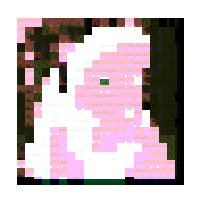
\includegraphics[scale=0.5]{pics/Alice/Nassaualice}}}
    = \vcenter{\hbox{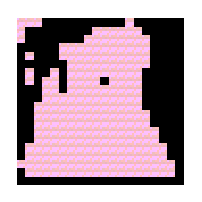
\includegraphics[scale=0.5]{pics/Alice/Nassaualice1}}}
    \oplus \vcenter{\hbox{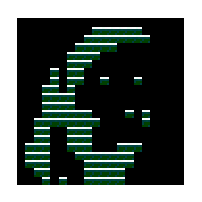
\includegraphics[scale=0.5]{pics/Alice/Nassaualice3}}}
    \oplus \vcenter{\hbox{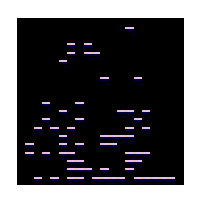
\includegraphics[scale=0.5]{pics/Alice/Nassaualice4}}}
    \oplus \vcenter{\hbox{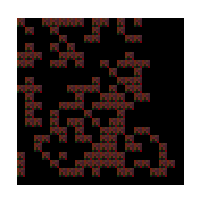
\includegraphics[scale=0.5]{pics/Alice/Nassaualice7}}} & \rotatebox[origin=c]{90}{\footnotesize(\textsc{Nassau})}\\
    %---------------- MDL4bmf
    &\approx
    \vcenter{\hbox{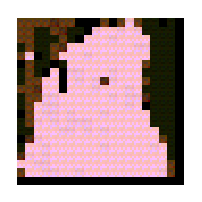
\includegraphics[scale=0.5]{pics/Alice/Mdl4bmfalice}}}
    = \vcenter{\hbox{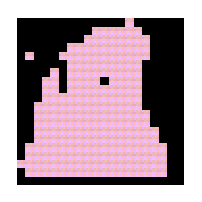
\includegraphics[scale=0.5]{pics/Alice/Mdl4bmfalice1}}}
    \oplus \vcenter{\hbox{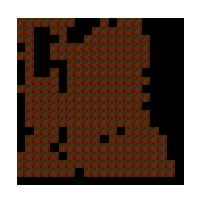
\includegraphics[scale=0.5]{pics/Alice/Mdl4bmfalice3}}}
    & \rotatebox[origin=c]{90}{\footnotesize (\textsc{Mdl4bmf}) }\\
    %---------------- Panda
    &\approx
    \vcenter{\hbox{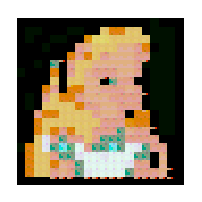
\includegraphics[scale=0.5]{pics/Alice/Pandaalice}}}
    = \vcenter{\hbox{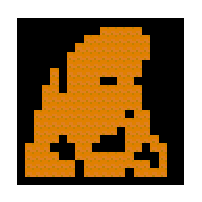
\includegraphics[scale=0.5]{pics/Alice/Pandaalice1}}}
    \oplus \vcenter{\hbox{
\includegraphics[scale=0.5]{pics/Alice/Pandaalice2}}}
    \oplus \vcenter{\hbox{
\includegraphics[scale=0.5]{pics/Alice/Pandaalice3}}}
    \oplus \vcenter{\hbox{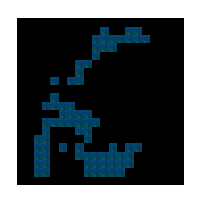
\includegraphics[scale=0.5]{pics/Alice/Pandaalice4}}}&\rotatebox[origin=c]{90}{ \footnotesize(\textsc{Panda+})}\\
    %-----------------Panpal---------------
     &\approx
     \vcenter{\hbox{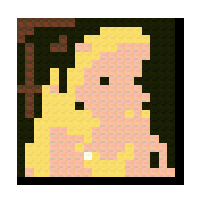
\includegraphics[scale=0.5]{pics/Alice/PanPalAlice}}}
    = \vcenter{\hbox{
\includegraphics[scale=0.5]{pics/Alice/PanPalAlice1}}}
    \oplus \vcenter{\hbox{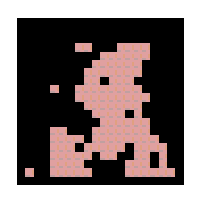
\includegraphics[scale=0.5]{pics/Alice/PanPalAlice4}}}
    \oplus \vcenter{\hbox{
\includegraphics[scale=0.5]{pics/Alice/PanPalAlice5}}}
    &\rotatebox[origin=c]{90}{\footnotesize(\textsc{Panpal}) }\\
     %-----------------Primp---------------
     &\approx
     \vcenter{\hbox{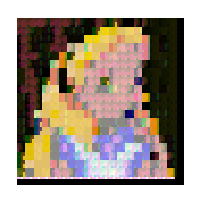
\includegraphics[scale=0.5]{pics/Alice/PrimpAlice}}}
    = \vcenter{\hbox{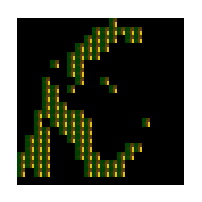
\includegraphics[scale=0.5]{pics/Alice/PrimpAlice1}}}
    \oplus \vcenter{\hbox{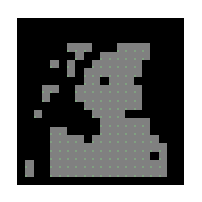
\includegraphics[scale=0.5]{pics/Alice/PrimpAlice3}}}
    \oplus \vcenter{\hbox{
\includegraphics[scale=0.5]{pics/Alice/PrimpAlice4}}}
    \oplus \vcenter{\hbox{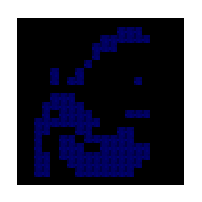
\includegraphics[scale=0.5]{pics/Alice/PrimpAlice6}}}& \rotatebox[origin=c]{90}{\footnotesize (\textsc{Primp}) }
  \end{align*}
  \caption{Reconstructions of the alice image and visualizations of the top-4 outer products. Best viewed in color.\label{fig:alice}}
\end{figure}

The original Alice image, as well as reconstructions $\theta(XY)$ and the top-4 tiles generated by \textsc{Nassau}, \textsc{Mdl4bmf}, \textsc{Panda+}, \textsc{Panpal} and \textsc{Primp}, are depicted in Figure~\ref{fig:alice}. 
Clearly, only \textsc{Panda+} and \textsc{Primp} select patterns, i.e., blocks of pixels which provide a reasonable reconstruction of the original image. \textsc{Panpal}'s tendency to underestimate the rank (choosing only three tiles) becomes apparent here again.
Regarding the figured structures, \textsc{Panda+}, \textsc{Panpal} and \textsc{Primp} discover a hair-related substructure, where the one found by \textsc{Primp} has the most distinctive contours, and \textsc{Panda+}, \textsc{Panpal} and \textsc{Primp} identify a face-related structure. The reconstructions and factors found by \textsc{Nassau} and \textsc{Mdl4bmf} are not easy to interpret without knowledge of the original image. 

\begin{figure}
  \begin{align*}
    &\vcenter{\hbox{\includegraphics[scale =0.2]{pics/SpaceInv/spaceInv}}}\\
    %---------------- MDL4bmf
    &\quad\approx
    \vcenter{\hbox{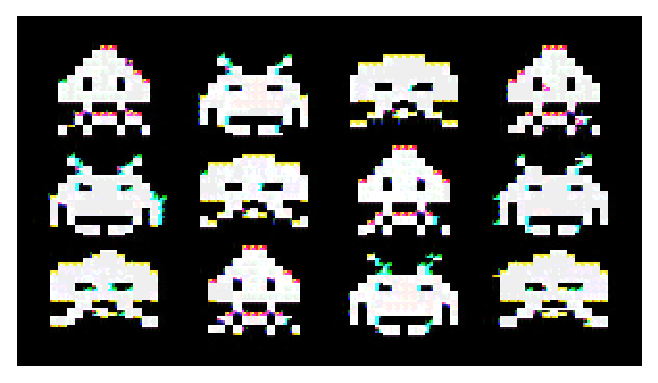
\includegraphics[scale =0.2]{pics/SpaceInv/NassauspaceInv}}}
    = \vcenter{\hbox{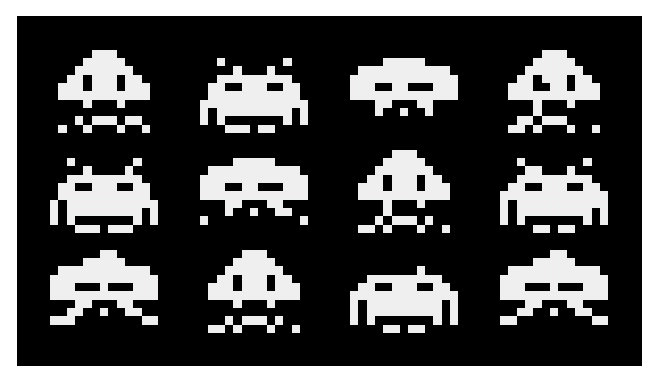
\includegraphics[scale =0.2]{pics/SpaceInv/NassauspaceInv1}}}
    \oplus \vcenter{\hbox{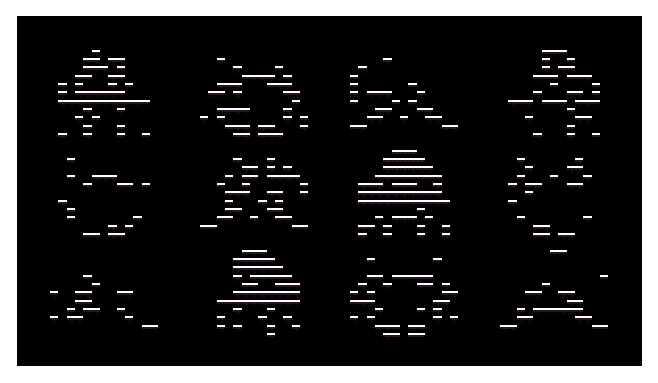
\includegraphics[scale =0.2]{pics/SpaceInv/NassauspaceInv2}}}
    \oplus \vcenter{\hbox{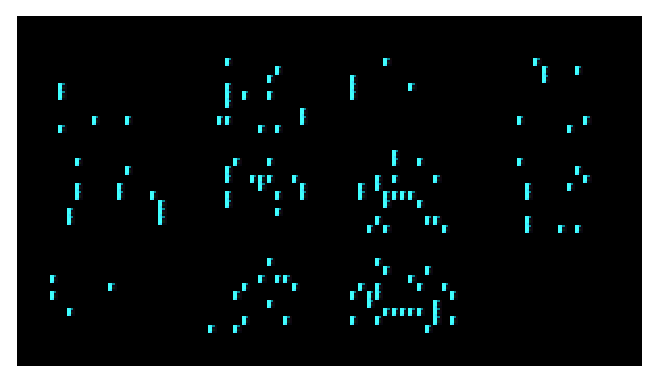
\includegraphics[scale =0.2]{pics/SpaceInv/NassauspaceInv8}}}
    \oplus \vcenter{\hbox{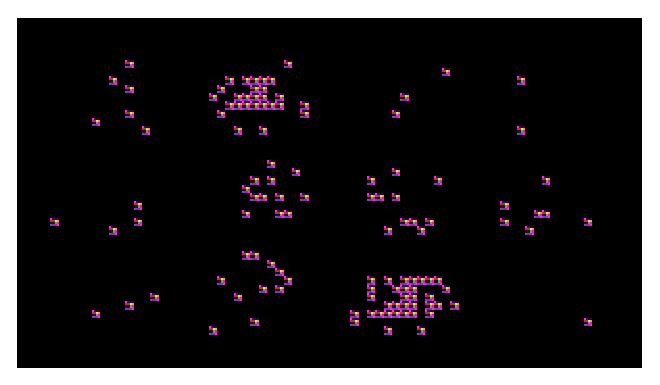
\includegraphics[scale =0.2]{pics/SpaceInv/NassauspaceInv11}}} & \rotatebox[origin=c]{90}{\footnotesize(\textsc{Nassau})}\\
    %---------------- MDL4bmf
    &\quad\approx
    \vcenter{\hbox{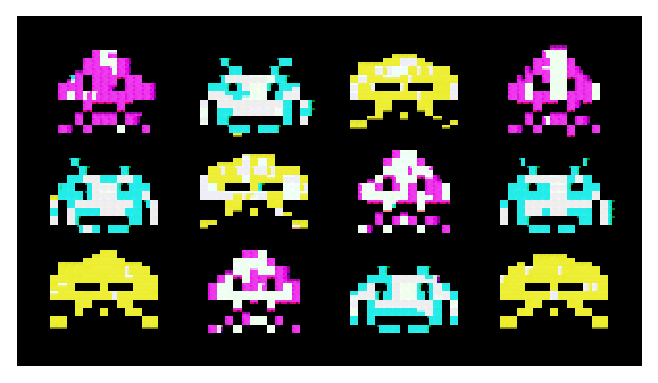
\includegraphics[scale =0.2]{pics/SpaceInv/Mdl4bmfspaceInv}}}
    = \vcenter{\hbox{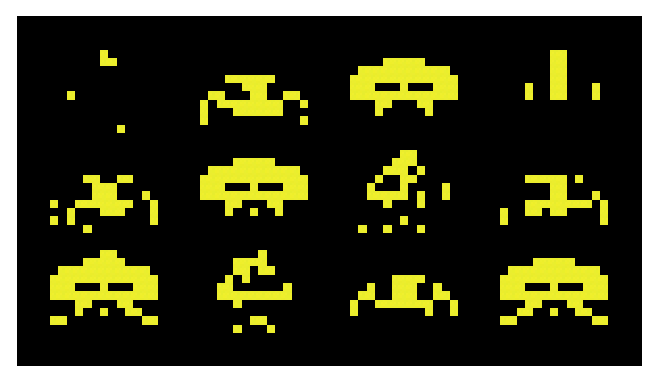
\includegraphics[scale =0.2]{pics/SpaceInv/Mdl4bmfspaceInv1}}}
    \oplus \vcenter{\hbox{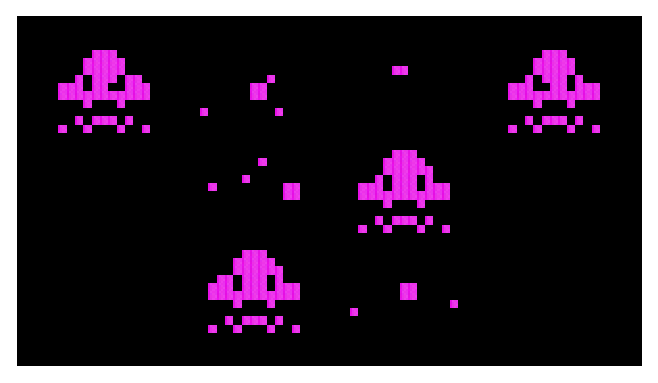
\includegraphics[scale =0.2]{pics/SpaceInv/Mdl4bmfspaceInv2}}}
    \oplus \vcenter{\hbox{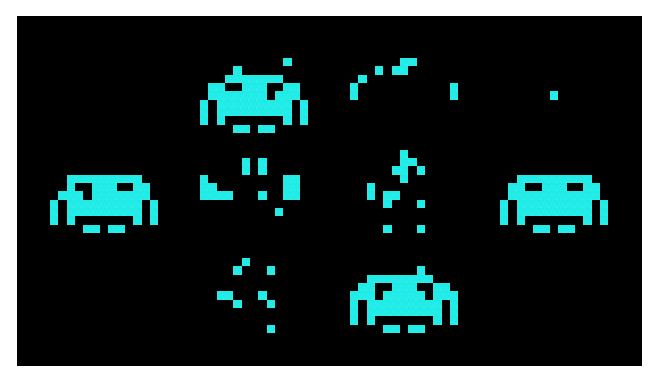
\includegraphics[scale =0.2]{pics/SpaceInv/Mdl4bmfspaceInv3}}}
    \oplus \vcenter{\hbox{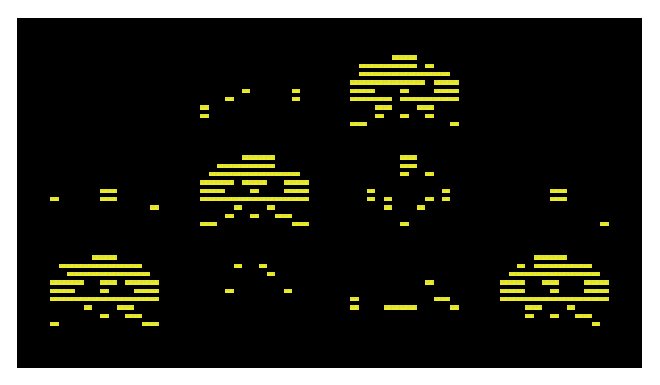
\includegraphics[scale =0.2]{pics/SpaceInv/Mdl4bmfspaceInv4}}} & \rotatebox[origin=c]{90}{\footnotesize (\textsc{Mdl4bmf}) }\\
    %---------------- Panda
    &\quad\approx
    \vcenter{\hbox{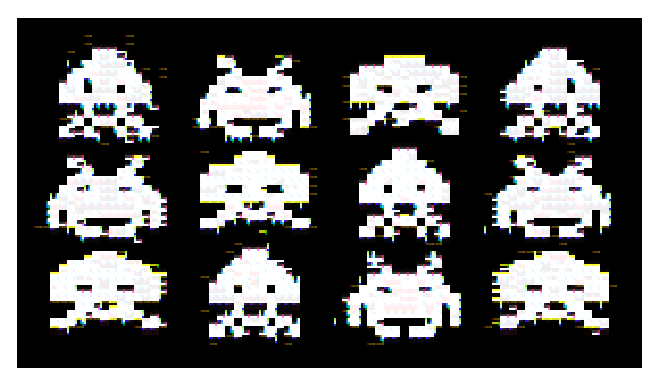
\includegraphics[scale =0.2]{pics/SpaceInv/PandaspaceInv}}}
    = \vcenter{\hbox{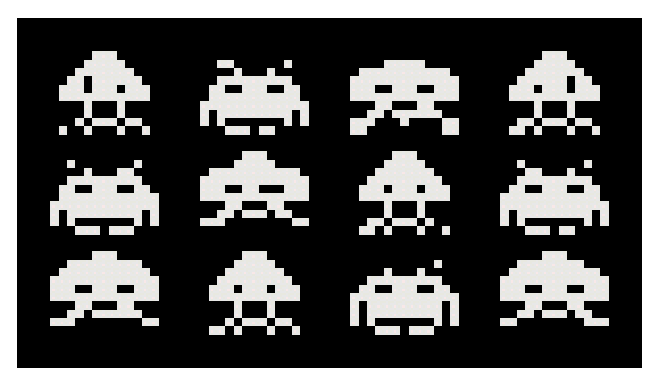
\includegraphics[scale =0.2]{pics/SpaceInv/PandaspaceInv1}}}
    \oplus \vcenter{\hbox{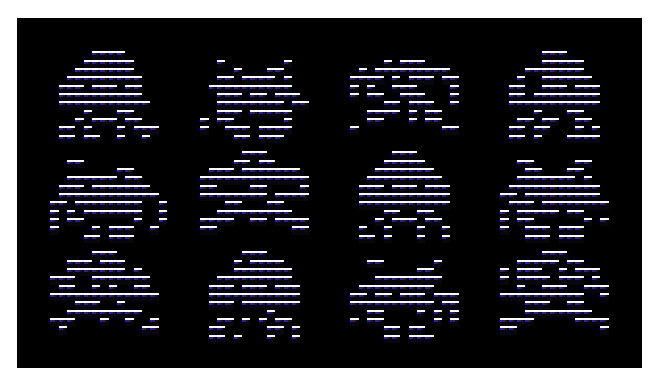
\includegraphics[scale =0.2]{pics/SpaceInv/PandaspaceInv2}}}
    \oplus \vcenter{\hbox{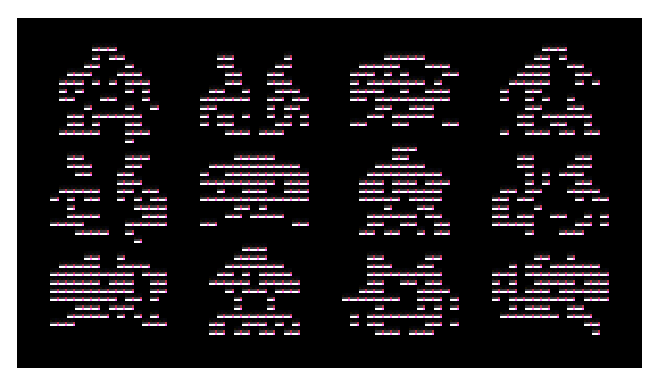
\includegraphics[scale =0.2]{pics/SpaceInv/PandaspaceInv3}}}
    \oplus \vcenter{\hbox{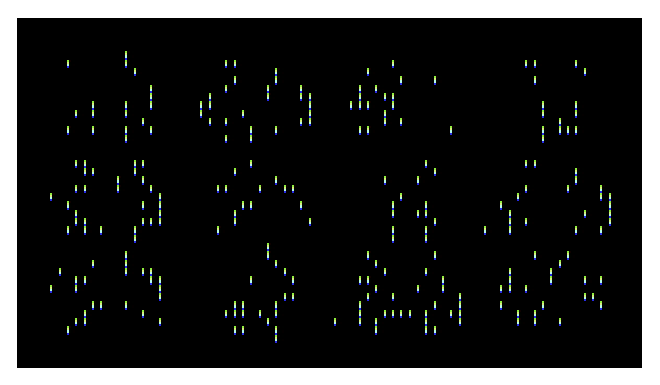
\includegraphics[scale =0.2]{pics/SpaceInv/PandaspaceInv4}}}&\rotatebox[origin=c]{90}{ \footnotesize(\textsc{Panda+})}\\
    %-----------------Panpal---------------
     &\quad\approx
     \vcenter{\hbox{\includegraphics[scale =0.2]{pics/SpaceInv/PanPalSpaceInv}}}
    = \vcenter{\hbox{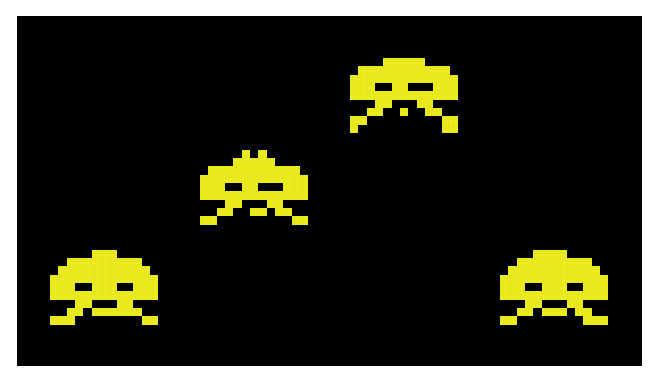
\includegraphics[scale =0.2]{pics/SpaceInv/PanPalSpaceInv1}}}
    \oplus \vcenter{\hbox{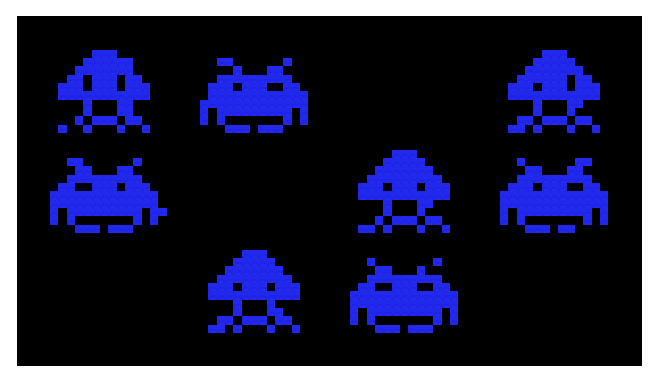
\includegraphics[scale =0.2]{pics/SpaceInv/PanPalSpaceInv2}}}&\rotatebox[origin=c]{90}{\footnotesize(\textsc{Panpal}) }\\
     %-----------------Primp---------------
     &\quad\approx
     \vcenter{\hbox{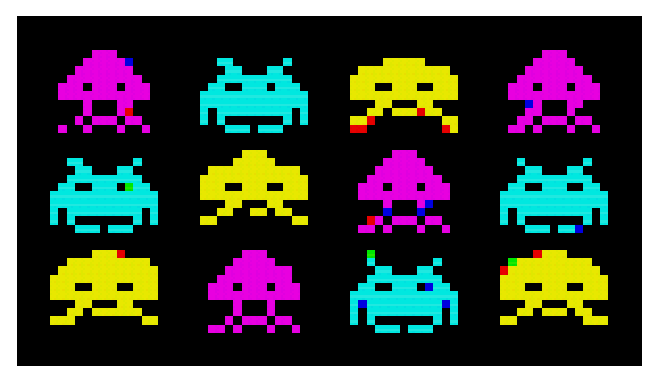
\includegraphics[scale =0.2]{pics/SpaceInv/PrimpSpaceInv}}}
    = \vcenter{\hbox{\includegraphics[scale =0.2]{pics/SpaceInv/PrimpSpaceInv1}}}
    \oplus \vcenter{\hbox{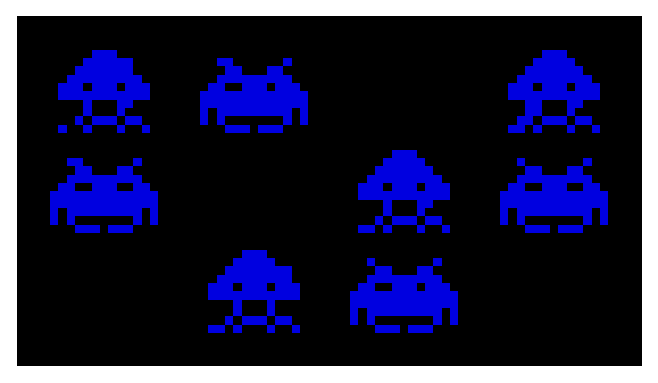
\includegraphics[scale =0.2]{pics/SpaceInv/PrimpSpaceInv2}}}
    \oplus \vcenter{\hbox{\includegraphics[scale =0.2]{pics/SpaceInv/PrimpSpaceInv3}}}& \rotatebox[origin=c]{90}{\footnotesize (\textsc{Primp}) }
  \end{align*}
  \caption{Reconstructions of the Space Invaders image and visualizations of the top-4 outer products. Best viewed in color.\label{fig:spaceInv}}
\end{figure}
Reconstruction results and top-4 patterns of the Space Invaders image are shown in Figure~\ref{fig:spaceInv}. All methods reconstruct at least the shape of the aliens. In terms of color, however, the results diverge. \textsc{Panda+} and \textsc{Nassau} interpret all colors as negative noise effects on the color white; white has a binary representation of $24$ ones. \textsc{Panpal} recovers the yellow color correctly and it extracts the full blue channel from the image---an identical pattern is also detected by \textsc{Primp}. \textsc{Primp} and \textsc{Mdl4bmf} reconstruct all three colors of the original image, yet the reconstruction of \textsc{Mdl4bmf} exhibits injections of white blocks. Hence, only \textsc{Primp} is capable to reconstruct the color information correctly. 

Having a look at derived tiles, the greedy processes of \textsc{Panda+} and \textsc{Nassau} become particularly visible; \textsc{Panda+} and \textsc{Nassau} overload the first factor with all the shape information. The remaining factors reduce the quantitative reconstruction error, but have no deeper interpretation. \textsc{Mdl4bmf} tries to model one type of aliens by each tile. Although this would result in a reasonable description of the image, the actual extraction of tiles suffers from the greedy implementation. We can see that, e.g., the first tile captures information about the yellow aliens as well as strayed parts of other aliens. This unfortunate allocation of tiles results in the injection of white blocks in the reconstruction image.  \textsc{Panpal} clearly separates yellow and blue aliens but interprets differences from the color blue to purple and to turquoise as noise. Finally, \textsc{Primp} separates by its tiles the three basic color channels which are actually used to mix the colors that appear in the original image. Hence, \textsc{Primp} achieves the factorization rank that corresponds to the natural amount of color concepts in the image, unlike all other competitors.

The results of this qualitive experiment particularly illustrates the benefits of a non-greedy minimization procedure. Even though \textsc{Panpal} is often not able to minimize the costs due to an underestimation of the rank, its categorization into tiles always yields interpretable parts.
%=====================
% Discussion
%=====================
\section{Discussion}
We introduce the minimization of description lengths for the derivation of Boolean matrix factorizations with an automatically determined rank by \textsc{PAL-Tiling}. Requiring that the description length has a smooth relaxed function, which combines the matrix factorization error with a regularizing function, \textsc{PAL-Tiling} minimizes the relaxed objective under convergence guarantees. %A thresholding to binary values according to the actual cost measure enables an automatic determination of the factorization rank.

Aiming at the robust identification of Boolean matrix factorizations in presence of various noise distributions, we consider two description lengths in this framework which defines two factorization algorithms. The first algorithm uses a simple $\ell 1$-norm regularization on the factor matrices and is called \textsc{Panpal}. The second minimizes the MDL-description length of the encoding by code tables as known from \textsc{Krimp} \citep{siebes2006item}. Foregoing the heuristics in computing the usage of codes, we extend the application of this encoding from pattern mining to Boolean matrix factorization and derive an upper bound which induces the relaxed objective. We refer to this instance of \textsc{PAL-Tiling} as \textsc{Primp}.

Our experiments on synthetically generated datasets show  that the quality of competing algorithms \textsc{Panda+}, \textsc{Mdl4bmf} and \textsc{Nassau} is sensitive towards multiple data generation parameters. The first of the two newly introduced algorithms, \textsc{Panpal}, regularly underestimates the true factorization rank. We have seen that this property can be beneficial in settings with large, overlapping tiles which induce dense datasets (cf.\@ Figure\@ \ref{fig:density}). In all other settings, the second algorithm \textsc{Primp} is able to detect the underlying structure, regardless of the considered distribution of noise or variations the factorization rank (cf.\@ Figures \ref{fig:noise810}-\ref{fig:rank}). 

A comparison of cost measures, as provided by the description lengths, on real-world datasets show that \textsc{Primp} also most often achieves lowest costs (cf.\@ Table\@ \ref{tbl:realWorldCosts}). With experiments based on images, we visualize the derived tiles under  presence of ambiguous factorization structures and special noise distributions (cf.\@ Figures \ref{fig:alice} and \ref{fig:spaceInv}). The quality of the reconstruction by established algorithms varies considerably between both images. On the contrary, \textsc{Panpal} and \textsc{Primp} provide solid representations of the original images. The extracted factors reveal a parts-based decomposition of the data (as known from nonnegative matrix factorizations), which allows for interpretation of the results. In the Space Invaders image (cf.\@ Figure\@ \ref{fig:spaceInv}), \textsc{Panpal} partitions the space invaders into those with a nonzero blue component in their color (rank-1 factorization 2) and those with a zero blue component in their color (rank-1 factorization 1). On the other hand, \textsc{Primp} divides the space invaders by the primary colors they contain (repeating each space invader exactly twice, hence finding structure in the data too, albeit a different structure from the one found by \textsc{Panpal}). From the Alice image (cf.\@ Figure~\ref{fig:alice}) particularly \textsc{Primp} manages to extract coherent factors representing the hair (rank-1 factorization 1) and the face (rank-1 factorization 4).

The implementation of the other popular cost measure, the Typed XOR DtM, is not readily realizable in \textsc{PAL-Tiling}. A real-valued relaxation of this description length involves the gamma function, which is not definable and thus, we cannot say whether this description length is a \KL function. Therefore, convergence to a local extremal point of the relaxed Typed XOR DtM function is not guaranteed in PALM. However, other description lengths are possibly worth exploring. For instance, a symmetric regularization of factor matrices appears to be more suitable in the scope of BMF, opposed to the asymmetric regularization implemented by \textsc{Primp}. The formulation of a description length which equally penalizes the model complexity in an encoding by code tables could simplify the implementation effort of \textsc{Primp} while maintaining the ability to suitably select the rank.
%Furthermore, the application of other penalizing functions $\phi$ is possible if the corresponding $\prox$-operator can be derived. 
%An analysis of the synergy between the penalizing function, the cost-measure and the thereby derived Boolean Matrix Factorization has the potential to show how the structure from arbitrary binary datasets can be robustly identified.